% Dokumentenart. Ersetze 12pt, falls die Schriftgröße anzupassen ist.
\documentclass[12pt]{scrartcl}

% Einbinden der Pakete, des Headers und der Formatierung.
% LaTeX Template für Abgaben an der Universität Stuttgart
% Autor: Sandro Speth
% Bei Fragen: Sandro.Speth@studi.informatik.uni-stuttgart.de
%-----------------------------------------------------------
% Modul fuer verwendete Pakete.
% Neue Pakete einfach einfuegen mit dem \usepackage Befehl:
% \usepackage[options]{packagename}
\usepackage[utf8]{inputenc}
\usepackage[T1]{fontenc}
\usepackage[ngerman]{babel}
\usepackage{lmodern}
\usepackage{graphicx}
\usepackage{float}
\usepackage[pdftex,hyperref,dvipsnames]{xcolor}
\usepackage{listings}
\usepackage[a4paper,lmargin={2cm},rmargin={2cm},tmargin={3.5cm},bmargin = {2.5cm},headheight = {4cm}]{geometry}
\usepackage{amsmath,amssymb,amstext,amsthm}
\usepackage[lined,algonl,boxed]{algorithm2e}
\usepackage{algorithmic}
\usepackage{multirow}
% alternative zu algorithm2e:
%\usepackage[]{algorithm} %counter mit chapter
%\usepackage{algpseudocode}
\usepackage{tikz}
\usepackage{hyperref}
\usepackage{url}
\usepackage[inline]{enumitem} % Ermöglicht ändern der enum Item Zahlen
\usepackage[headsepline]{scrlayer-scrpage} 
\usepackage{csquotes}
\pagestyle{scrheadings} 
\usetikzlibrary{automata,positioning,shapes.geometric,trees}

% LaTeX Template für Abgaben an der Universität Stuttgart
% Autor: Sandro Speth
% Bei Fragen: Sandro.Speth@studi.informatik.uni-stuttgart.de
%-----------------------------------------------------------
% Modul beinhaltet Befehl fuer Aufgabennummerierung,
% sowie die Header Informationen.

% Überschreibt enumerate Befehl, sodass 1. Ebene Items mit
\renewcommand{\theenumi}{(\alph{enumi})}
\renewcommand{\theenumii}{(\roman{enumii})}
% (a), (b), etc. nummeriert werden.
\renewcommand{\labelenumi}{\text{\theenumi}}
\renewcommand{\labelenumii}{\text{\theenumii}}

% Counter für das Blatt und die Aufgabennummer.
% Ersetze die Nummer des Übungsblattes und die Nummer der Aufgabe
% den Anforderungen entsprechend.
% Gesetz werden die counter in der hauptdatei, damit siese hier nicht jedes mal verändert werden muss
% Beachte:
% \setcounter{countername}{number}: Legt den Wert des Counters fest
% \stepcounter{countername}: Erhöht den Wert des Counters um 1.
\newcounter{sheetnr}
\newcounter{exnum}

% Befehl für die Aufgabentitel
\newcommand{\exercise}[1]{\section*{Exercise \theexnum\stepcounter{exnum}: #1}} % Befehl für Aufgabentitel

% Formatierung der Kopfzeile
% \ohead: Setzt rechten Teil der Kopfzeile mit
% Namen und Matrikelnummern aller Bearbeiter
\ohead{Hui Zeng}
% \chead{} kann mittleren Kopfzeilen Teil sezten
% \ihead: Setzt linken Teil der Kopfzeile mit
% Modulnamen, Semester und Übungsblattnummer
\ihead{Cloud Computing\\
Summer semester 2021\\
Lecture Notes Summary}

\definecolor{comments}{rgb}{0.41,0.54,0.21}
\definecolor{code}{rgb}{0,0,0}
\definecolor{keyword}{rgb}{0.77,0.48,0.57}
\definecolor{number}{rgb}{0.153,0.5,0}
\definecolor{codeBack}{rgb}{0.85,0.85,0.85}
\definecolor{string}{rgb}{0.81,0.57,0.47}

\lstdefinestyle{stdCode}{
	backgroundcolor=\color{codeBack},   
	commentstyle=\color{comments},
	literate=*{0}{{\textcolor{number}{0}}}{1}%
         {1}{{\textcolor{number}{1}}}{1}%
         {2}{{\textcolor{number}{2}}}{1}%
         {3}{{\textcolor{number}{3}}}{1}%
         {4}{{\textcolor{number}{4}}}{1}%
         {5}{{\textcolor{number}{5}}}{1}%
         {6}{{\textcolor{number}{6}}}{1}%
         {7}{{\textcolor{number}{7}}}{1}%
         {8}{{\textcolor{number}{8}}}{1}%
         {9}{{\textcolor{number}{9}}}{1}%
         {.0}{{\textcolor{number}{.0}}}{1}% Following is to ensure that only periods
         {.1}{{\textcolor{number}{.1}}}{1}% followed by a digit are changed.
         {.2}{{\textcolor{number}{.2}}}{1}%
         {.3}{{\textcolor{number}{.3}}}{1}%
         {.4}{{\textcolor{number}{.4}}}{1}%
         {.5}{{\textcolor{number}{.5}}}{1}%
         {.6}{{\textcolor{number}{.6}}}{1}%
         {.7}{{\textcolor{number}{.7}}}{1}%
         {.8}{{\textcolor{number}{.8}}}{1}%
         {.9}{{\textcolor{number}{.9}}}{1}%
         {\ }{{ }}{1}% handle the space
         ,%
	keywordstyle=\color{keyword},
	numberstyle=\tiny\color{number},
	stringstyle=\color{string},
	basicstyle=\ttfamily\scriptsize,
	breakatwhitespace=false,         
	breaklines=true,                 
	captionpos=b,                    
	keepspaces=true,                 
	numbers=left,                    
	numbersep=5pt,                  
	showspaces=false,                
	showstringspaces=false,
	showtabs=false,                  
	tabsize=2
}

\lstset{
	style=stdCode, language=Java,
  	literate={ö}{{\"o}}1
           {ä}{{\"a}}1
           {ü}{{\"u}}1
}

\tikzset{triangle/.style = {regular polygon, regular polygon sides=3 },
node rotated/.style = {rotate=180},
border rotated/.style = {shape border rotate=180},
astTerminal/.style = {regular polygon, regular polygon sides=3, inner sep=2.5pt, shape border rotate=180},
astLabel/.style = {right=3pt,font=\footnotesize\itshape},
astValue/.style = {below=5pt},
astLine/.style = {edge from parent fork down}
}
\graphicspath{{bilder/}}

\usepackage{eurosym}

% Counter für das Blatt und die Aufgabennummer.
\setcounter{sheetnr}{0} % Nummer des Übungsblattes
\setcounter{exnum}{1} % Nummer der Aufgabe

\newcommand*\circled[1]{\tikz[baseline=(char.base)]{
		\node[shape=circle,draw,inner sep=2pt] (char) {#1};}}     % number in circles
% Beginn des eigentlichen Dokuments
\begin{document}
	\pagenumbering{roman}
	\title{Business Analytics}
\author{Hui Zeng \thanks{All notes are summarized from the lecture and tutorial materials provided by Prof. Martin Bichler and his DSS team. Images are retrieved from the lecture as well as tutorial slides.}}
\date{Winter Semester 2020-2021}
\maketitle

\newpage
	\newpage
	\setcounter{tocdepth}{2}
	
	\tableofcontents
	\newpage
	\flushleft
	
	\pagenumbering{arabic}
	\section{Introduction}
Different IT-trends boosts the need for cloud computing:
\begin{itemize}
	\item Outsourcing, either infrastructure or management
	\item IT as a service: pay per use
	\item Re-centralization of data: similar to data centers, cloud be provided as a central place for data storage.
	\item Resource sharing instead of over-provisioning: same resource can be used for multiple purposes
	\item Server consolidation: instead of having multiple physical servers, with each dedicated to a certain service, servers are virtualized and put on one/reduced number of physical machines.     
	\item Scalable computing
	\item Application dynamism: amount of request on web changes over time.
	\item Green computing, big data, stream processing, IoT, machine learning, etc.
\end{itemize}

\paragraph{Cloud Computing} the definition is mainly divided by
\begin{itemize}
	\item ubiquitous, convenient, on-demand network access to a \textbf{shared pool of configurable computing resources} (eg: networks, servers, storage, applications, services)
	\item resources can be \textbf{rapidly provisioned} and released with \textbf{minimal management effort} or service provider interaction
	\item cloud model is composed of 
	\begin{itemize}		
		\item 3 service models
		\item 4 deployment models
		\item 5 essential characteristics
	\end{itemize}
\end{itemize}

\subsection{3 Service Models: IaaS, PaaS and SaaS}
Three service models, ranking from outsourcing the least to the most: IaaS $\rightarrow$ PaaS $\rightarrow$ SaaS.

\subsubsection{IaaS: Infrastructure as a Service}
\begin{itemize}
	\item Offering: provision processing, storage, networks, other fundamental computing resources
	\item Rights as consumer: 
	\begin{itemize}
		\item deploy and run \textbf{arbitrary} software, including \textbf{operating systems and applications}
		\item control over OS, storage, deployed applications
		\item limited control of select networking components
	\end{itemize}
	\item No control as consumer:
	\begin{itemize}
		\item underlying cloud infrastructure
	\end{itemize}
	
	
\end{itemize}
\subsubsection{PaaS: Platform as a Service}
\begin{itemize}
	\item Offering: application infrastructure services(eg: development platforms, libraries, tools, databases) through client interface
	\item Rights as consumer:
	\begin{itemize}
		\item limited user-specific application configuration settings
	\end{itemize}
	\item No control as consumer:
	\begin{itemize}
		\item underlying cloud infrastructure
		\item network, servers, storage, OS
		\item individual application capabilities
	\end{itemize}
	\item Example: MS Azure, Amazon FaaS, Google application engine
\end{itemize}
\subsubsection{SaaS: Software as a Service}
\begin{itemize}
	\item Offering: provider's applications on cloud through client interface
	\item Rights as consumer:
	\begin{itemize}
		\item limited user-specific application configuration settings
	\end{itemize}
	\item No control as consumer:
	\begin{itemize}
		\item underlying cloud infrastructure
		\item network, servers, OS, storage
		\item individual application capabilities
	\end{itemize}
\end{itemize}
\begin{figure}[H]
	\centering
	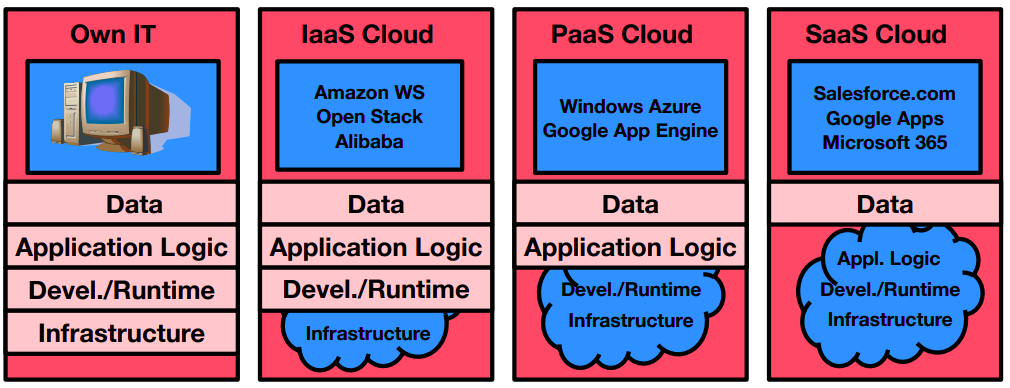
\includegraphics[width=\textwidth]{servicemodels.png}
	%\caption{Comparison over the service models}
\end{figure}
\begin{figure}[H]
	\centering
	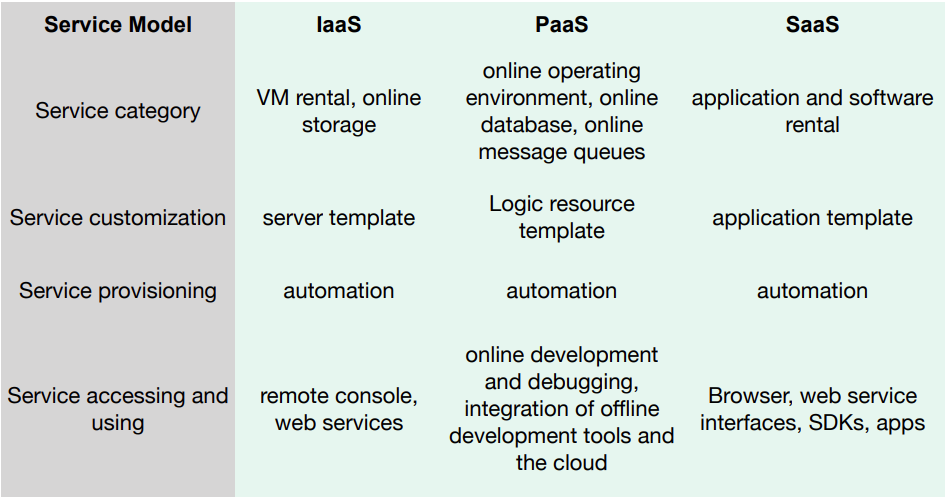
\includegraphics[width=0.8\textwidth]{servicemodel1.png}
	%\caption{Comparison over the service models}
\end{figure}\begin{figure}[H]
\centering
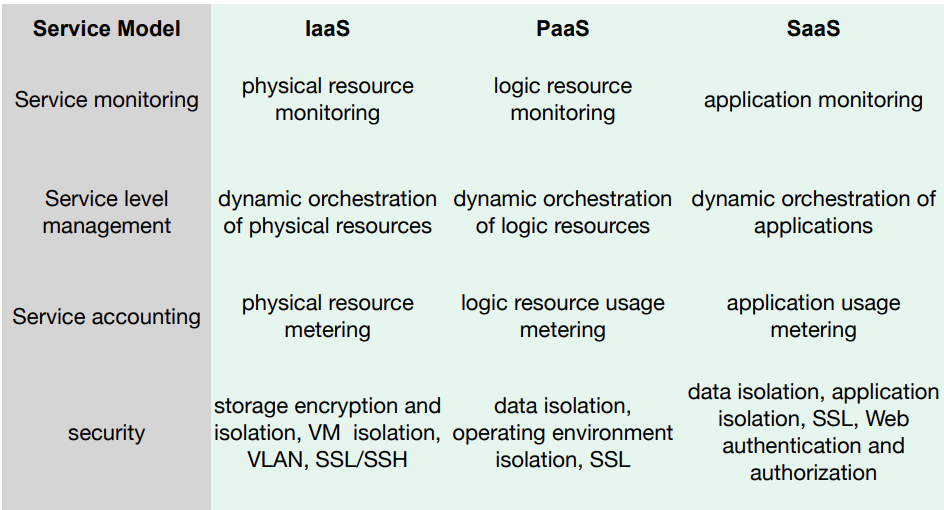
\includegraphics[width=0.8\textwidth]{servicemodel2.png}
%\caption{Comparison over the service models}
\end{figure}
\subsection{4 Deployment Models: Private, Community, Public, Hybrid}
\begin{itemize}
	\item Private Cloud:
	\begin{itemize}
		\item service offered \textbf{via private network} for \textbf{single client}.
	\end{itemize}
	\item Community Cloud:
	\begin{itemize}
		\item service offered to \textbf{a specific group of clients}.
	\end{itemize}
	\item Public Cloud:
	\begin{itemize}
		\item service offered \textbf{over Internet via Web-application} or third-party provider for \textbf{everyone}.
	\end{itemize}
	\item Hybrid Cloud: combination of public and private cloud.
\end{itemize}

\subsection{5 Essential Characteristics}
\begin{itemize}
	\item \textbf{on-demand self-service}: 
	\begin{itemize}
		\item able to \textbf{provision computing capabilities} unilaterally(no interaction required with provider).
	\end{itemize}
	
	\item \textbf{broad network access}: 
	\begin{itemize}
		\item capabilities can be available and accessed through by \textbf{diversely thin or thick client platforms} (mobile, tablets, cable, etc.)
	\end{itemize}
	
	\item \textbf{resource pooling}: 
	\begin{itemize}
		\item \textbf{multi-tenant model} is used, multiple customers shares the computing capabilities at the same time, according to their self-customized demand. Specification of resource location can be possible at higher abstraction level.
	\end{itemize}
	 
	\item \textbf{rapid elasticity}: 
	\begin{itemize}
		\item computing capabilities can be \textbf{elastically provisioned and released} in any quantity at any time. The process can be automated or scaled according to dynamic demand.
	\end{itemize}
	\item \textbf{measured service}: 
	\begin{itemize}
		\item automatically control and optimize resource use by \textbf{leveraging a metering capability}. Resource usage can be monitored, controlled and reported.
	\end{itemize}
\end{itemize}


\subsection{Pros \& Cons of Clouds}
\begin{itemize}
	\item Advantages:

\begin{itemize}
	\item scalability, elasticity
	\item rapid deployment
	\item no capital investment for physical resources
	\item outsourcing of infrastructure management
	\item limited access to on-premise servers
	\item fault tolerance: multiple servers have data replicas, if one node fails, other nodes will replace.
	\item collaboration
\end{itemize}
	\item Disadvantages:
	\begin{itemize}
		\item no control over security, based on ''trust''.
		\item no control over hardware/infrastructure
		\item vendor lockin: service is not standardized, not compatible to other vendors.
		\item cost on monthly fees: if demand for same computational power is constant, fee may be higher than building own hardware. Only recommendable for dynamic demand.
		\item breaking SLAs: your performance may be influenced by other tenants(multi-tenant model).
	\end{itemize}
\end{itemize}
	\section{Base Technologies of Clouds}
\subsection{Process Technology}
\paragraph{Production} the processors are produced from semi-conductor materials. It's primarily produced on a \textbf{waver} consisting of a lot of chips. Later the waver is cut after the production process. Individual chips will be packaged into the system.

\paragraph{Transistor} 
\begin{itemize}
	\item traditional 2D planar transistor: a 2D-planar structure, the gate controls how much current flows from source through the drain.
	\item 3D tri-gate transistor \textbf{FinFET}: conducting channels on 3 sides with a \textbf{vertical fin structure}. The width of a Fin is \textbf{10nm}, and it keeps shrinking.
\end{itemize}
The smaller the structure gets, the more transistors fit on the same space, the faster the transistor gets.

\subsection{Processor Architecture}

\subsubsection{CPU}
\begin{itemize}
	\item current state of CPU development:
	\begin{itemize}
		\item increase in transistors: up to 10nm or even 5nm.
		\item stop in increase of clock speed: up to 4GHz. Limitation: cooling. (the faster the clock speed, the more energy consumed, the hotter) 
		\item continuous need of performance improvement: parallelism on the chip, since halt in clock speed.
	\end{itemize}
	\item trends in CPU development:
	\begin{itemize}
		\item multi-core processors: parallelism
		\item SIMD support (Single Instruction, Multiple Data): parallelism inside of a single instruction, computation of vectors of values in parallel.
		\item combination of core private and shared caches:
		\begin{itemize}
			\item data saved in cache for repeated operations
			\item with multiple caches, cores can communicate. However, this may disturb the usage of cache.
			
		\end{itemize}
		\item hardware support for energy control: \textbf{dynamic voltage and frequency scaling}  
		\begin{itemize}
			\item chips work in a dynamic frequency controlled by hardware according to the need of the running software. 
			\item It checks whether operations are memory-bound or compute-bound.
		\end{itemize}
		   
		\item 64-bit architectures
		  
	\end{itemize}
	\item challenge: the \textbf{memory hierarchy}
	\begin{itemize}
		\item access to the main memory is slow, involving several hundreds of cycles for CPU, while each of these cycles can be responsible for multiple operations.
		
		$\rightarrow$ save such cycles for accessing data but keep the \textbf{data near to execution}.
		\item \textbf{Level-1 Instruction \& Data Cache}: fastest, but too slow to feed all data in large size. (64 Bytes: 8 double precision values, 64 bit long values)
		\item \textbf{Level-2 Unified Cache}: not separated, access better. 
		\item \textbf{Translation Lookaside Buffer (TLB)}: translates virtual addresses into physical addresses and loads into main memory, it only stores the \textbf{most recent translation}, no need to lookup constantly.
	\end{itemize}
	\begin{figure}[H]
		\centering
		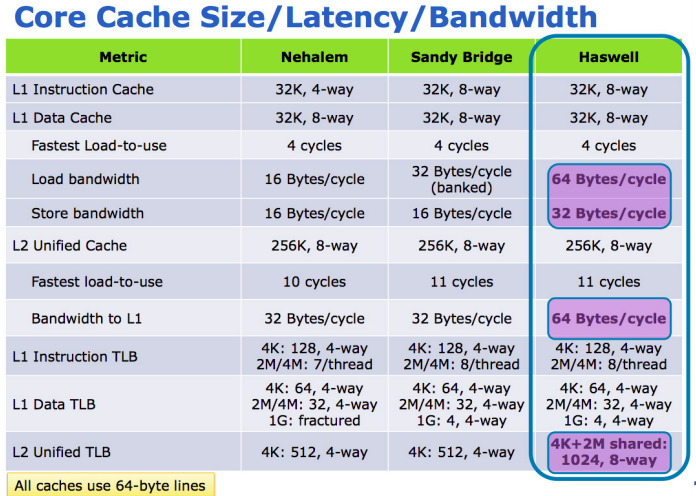
\includegraphics[width=0.65\textwidth]{memhier.png}
	\end{figure}
\end{itemize}

\subsubsection{Skylake Architecture} 

\begin{figure}[H]
	\centering
	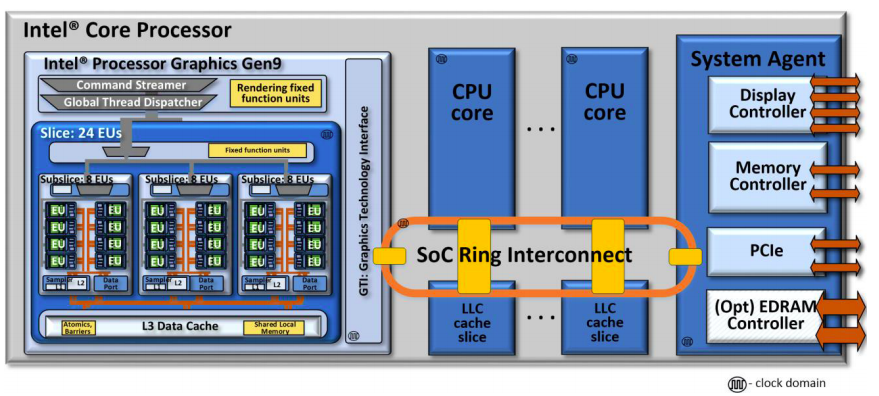
\includegraphics[width=0.7\textwidth]{skylake.png}
\end{figure}
The archiecture of a processor (one chip)
\begin{itemize}
	\item graphic processor: accelerator for specified computation
	\item system agent: support structures (eg: display controller, memory controller, PCIe for I/O, EDRAM controller)
	\item CPU cores: homogeneous cores with a \textbf{private cache each}.
	\item LLC cache slice: each slice cache is associated to each CPU core. 
	\begin{itemize}
		\item If core misses information in its private cache: through interconnect, it checks which slice cache contains the info, then it propagates to the cache associated the CPU core and returns the info back to the CPU.
	\end{itemize}
	
	\item SoC Ring interconnect: all parts are connected by a ring bust.
	\begin{itemize}
		\item if CPU writes to I/O device -- PCIe, it first puts information onto the bust, then it propagates into the PCIe and is written to the disk.
	\end{itemize}
\end{itemize}
$\rightarrow$ the \textbf{interconnect ring} is the \textbf{bottleneck} for increasing the cores.

$\rightarrow$ alternatives: Xeon Phi

\subsubsection{Xeon Phi Architecture} 
\begin{figure}[H]
	\centering
	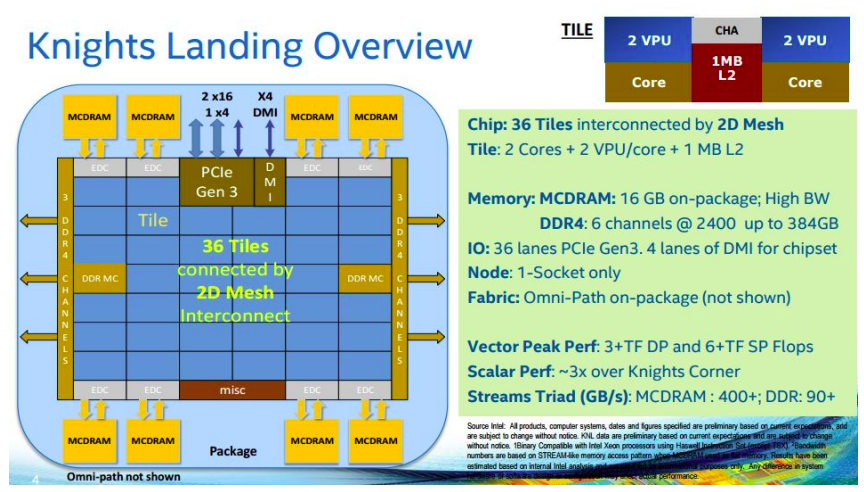
\includegraphics[width=0.7\textwidth]{xeonphi.png}
\end{figure}
\begin{itemize}
	\item Goal: allows significantly \textbf{more cores} in a single processor, in a single CPU die.
	\item Idea: 
	\begin{itemize}
		\item the die is organized into a \textbf{tile-architecture}.
		\item 36 compute tiles are connected through a \textbf{2D mesh network} $\rightarrow$ connection between tiles in both x- and y-direction.
		\item each tile has 2 cores $\rightarrow$ \textbf{72 cores} in total
	\end{itemize}
	\item Tile structure:
	\begin{itemize}
		\item 2 cores
		\item 2 VPUs (Vector Processing Unit) for each core $\rightarrow$ 4 in total per tile.
		\item L2 cache: shared between the cores, but as a private cache for each tile. 
		
		$\rightarrow$ multiple copies of an address can be in different private L2 caches of different tiles, which \textbf{must be coherent}.
		\item CHA (Caching Hold Agent): responsible for the \textbf{coherence}. It's connected to each tile, keeping track of the status of the copies by implementing a \textbf{coherence protocol}. 
	\end{itemize}
	\item Memory: 
	\begin{itemize}
		\item DDR4 memory
		\item \textbf{MCDRAM}-- Multi-channel DRAM, \textbf{high bandwidth}(450 GB/s)
		
		Memory modes:
		\begin{itemize}
			\item flat mode: all MCDRAM is used as \textbf{physical address}. Data structure can explicitly choose between MCDRAM or DDR. 
			\item cache mode: all MCDARM is used as \textbf{L3 cache}. physical addresses only on DDR. If data is being processed from DDR, it's mapped to MCDRAM.
			\item hybrid mode: combination of flat and cache mode. Part of MCDRAM is used as \textbf{L3 cache}, the other as \textbf{physical addresses}.
		\end{itemize}
		\begin{figure}[H]
			\centering
			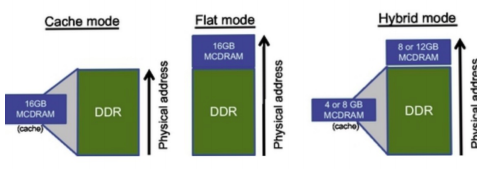
\includegraphics[width=0.65\textwidth]{memorymodes.png}
		\end{figure}
	\end{itemize}	
\end{itemize}

\subsubsection{Processors for mobile devices: ARM}
\begin{figure}[H]
	\centering
	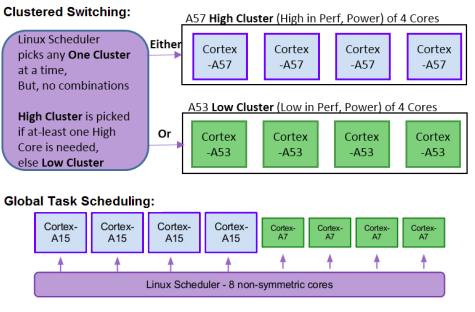
\includegraphics[width=0.65\textwidth]{arm.png}
\end{figure}
\begin{itemize}
	\item \textbf{Big Little Principle}
	\begin{itemize}
		\item Combination of \textbf{high clusters} and \textbf{low clusters}, controlled by clustered switching. 
		\begin{itemize}
			\item high cluster: high in performance
			\item low cluster: low in performance, but energy efficient
			\item only \textbf{one cluster} at a time, \textbf{no combinations}.
		\end{itemize}
		\item Global task scheduling: tasks are scheduled according to the requirement between 2 clusters.
	\end{itemize}
	\item Use-cases: Apple Processor A14 (2 high performance Firestorm, 2 energy-efficient Icestorm)
\end{itemize}


\subsection{Accelerator Programming}
\begin{itemize}
	\item Motivation: 
	\begin{itemize}
		\item increase computational speed and reduce energy consumption
		
		$\rightarrow$ achieved by \textbf{specialization} in operations/on-chip communication/memory accesses
		
		$\rightarrow$ \textbf{accelerator}
	\end{itemize}
	\item Types:
	\begin{itemize}
		\item GPGPU (General Purpose Graphic Processors)
		\item FPGA
		\item standard cores
	\end{itemize}
	\item Designs:
	\begin{itemize}
		\item CPU with accelerators attached: computation can be offloaded onto the accelerator.
		\item accelerators-only design
		\item accelerator booster: a collection of accelerators as a separate part from the whole system. Jobs can be computed by these accelerators when necessary. Accelerator booster can be shared among parallel jobs.
	\end{itemize}
	
\end{itemize}

\subsubsection{Graphic Processing Units (GPU)}
\begin{itemize}
	\item Usage: 
	\begin{itemize}
		\item visualization
		\item \textbf{general processing} (NVIDIA)
	\end{itemize}
	\item Parallelism: multi-threading, MIMD, SIMD
	\item Challenges:
	\begin{itemize}
		\item a \textbf{specialized programming interface} for the GPGPU needed (eg: CUDA from NVIDIA)
		\item \textbf{scheduling coordination} on system processor and GPU
		\item \textbf{transfer of data} between system memory and GPU memory
	\end{itemize} 
	\item example: NVIDIA Tesla P100
\end{itemize}

\paragraph{NVIDIA Tesla P100}
\begin{itemize}
	\item GP100 (GPU):
	\begin{itemize}
		\item L2 cache: shared among all compute units --  streaming multi-processor
		\item NVLink: able to connect multiple GPGPUs together
		\item memory controller: access to high bandwidth memory
		\item 6 Graphic Processing Clusters(GPC)
			\begin{itemize}
				\item 10 Streaming Multi-Processor each GPC, 60 in total
				\item 5 Textural Processing Clusters (TPC), 1 for 2 SM, 30 in total
			\end{itemize}
		\end{itemize}

		\item High Bandwidth Memory (HBM)
		\begin{itemize}
			\item \textbf{vertical stacks} of memory dies connected by microscopic wires
		
			$\rightarrow$ near and tight connection between memories
			\item 180 GB/s per stack bandwidth
		\end{itemize}
\end{itemize}

$\rightarrow$ good for data parallel processing like vector processing.

\subsubsection{Field Programmable Gate Arrays (FPGA)}
\begin{itemize}
	\item hardware which is programmable
	\item Consist of:
	\begin{itemize}
		\item \textbf{array of logic gates} to implement \textbf{hardware-programmed special functions}
		\item \textbf{specialized functional units} (eg: signal processors, multipliers)
		\item static \textbf{memory}
	\end{itemize}
	\item programmed in VHDL: the program describe functions to be executed, it will then be translated into look-up tables, which are put into the logic gates
	\item Use-case:
	\begin{itemize}
		\item as \textbf{accelerator} for specialized computations
		\item \textbf{filtering} for databases
		\item as \textbf{switches, routers} for communication
		\item \textbf{preprocessing}: I/O hardware of FPGA accesses the DDR, local computation can be organized in the pipeline of FPGA. Local preprocessing will be done on FPGA and the output will be sent ot external processor via PCIe.
	\end{itemize}
	\item examples: Altera, Xilinx
\end{itemize}

\subsection{Architecture for Parallelism: Shared Memory Systems}
\begin{itemize}
	\item Idea: 2 architectures to \textbf{achieve parallelism}, which is combining multiple processors together for computation. 
	\begin{itemize}
		\item shared memory system
		\item distributed memory system
	\end{itemize}
	\item \textbf{Non-Uniform Memory Access (NUMA)}:
	\begin{itemize}
		\item \textbf{multiple CPU} with multiple cores are connected through \textbf{single physical address} space.
		
		$\rightarrow$ access time depends on the \textbf{distance to the physical address} (memory)
		
		$\rightarrow$ CPU accesses either local(near) or remote memory $\rightarrow$ locate the memory near for fast access.
	\end{itemize}
	\paragraph{Example: SuperMUC}
	
	\begin{itemize}
		\item 2 multi-core processors(Sandy Bridge) with 32GB memory in total
		\item each processor can access to all 32GB memory, \textbf{however access time differs}
		\item \textbf{Latency}
		\begin{itemize}
			\item local: $\sim$50ns, $\sim$135 cycles
			\item remote: $\sim$90ns, $\sim$240 cycles
		\end{itemize}
		
	\end{itemize}
	\begin{figure}[H]
		\centering
		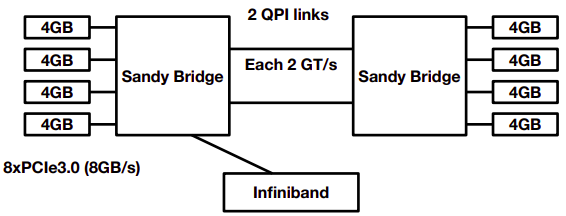
\includegraphics[width=0.65\textwidth]{numa.png}
	\end{figure}

	\item Programming interfaces for Shared Memory Systems
	\begin{itemize}
		\item explicit threading
		\item automatic parallelization: sequential code is given to compiler, which \textbf{automatically} parallelize the work among available CPUs.
		\item OpenMP: directive-based parallel programming, parallel computations are \textbf{explicitly expressed}.
	\end{itemize}
	\item Challenges in parallel computing:
	\begin{itemize}
		\item explicit synchronization needed.
		\item \textbf{cocurrency bugs}: the outcome of the computation depends on the speed of access to the memory $\rightarrow$ non-deterministic results possible.
		\item control of \textbf{data locality}
	\end{itemize}
\end{itemize}

\subsection{Architecture for Parallelism: Distributed Memory Systems}
\begin{itemize}
	\item Characteristics
	\begin{itemize}
		\item \textbf{Coupling} of individual nodes via network: processor only have access to the memory in node.
		\item \textbf{no shared} physical address space
		\item communication between nodes: transfer of \textbf{messages}
	\end{itemize}
	\item Programming in Distributed Memory Systems: \textbf{more difficult} than shared memory systems.
	\begin{itemize}
		\item + : \textbf{rare race conditions} $\rightarrow$ cocurrency bugs low.
		\item -- : Message Passing Interface(MPI), have to explicitly decompose or insert message passing $\rightarrow$ more difficult to program.
		\item Process to Process communication and collective operations
	\end{itemize}
	\item Challenges: 
	\begin{itemize}
		\item \textbf{more difficult} to programm than shared memory systems
		\item \textbf{expensive communication}, much slower than access to memory.
		$$t(message) = \text{startup time} + \frac{\text{message size}}{\text{bandwidth}}$$
		\begin{itemize}
			\item communication with one large message is more efficient than multiple small messages (startup time)
			\item mapping onto processors has performance impact. Communication may not need to go through the entire but locally. (eg: 2D mesh network)
		\end{itemize}
	\end{itemize}
\end{itemize}

\subsection{Data Center Networks}
Inside the data center, the \textbf{servers} are connected by \textbf{LAN}-- Local Area Network. Each \textbf{server} is connected to a \textbf{switch}. The \textbf{switches} are connected, which allows \textbf{communication between the servers}. \\ \ \\

Multiple \textbf{LANs} are possible in a data center. The \textbf{LANs} can be connected through a \textbf{router}. A router is based on a IP-address, it can make decisions depending on the IP-address (eg: receiver of message). \\ \ \\

The \textbf{routers} in the data center can be connected to a \textbf{WAN}-- Wide Area Network, the internet. The \textbf{WAN} can be connected to a \textbf{local router}, which a client has access to . This is the \textbf{last mile} to reach the client, frequently \textbf{radio network} is used -- WLAN or GSM.

\subsubsection{Different Networks}
\begin{itemize}
	\item Types:
	\begin{itemize}
		\item WAN -- Wide Area Networks
		\begin{itemize}
			\item homogeneous base technology (opto-electronic)
		\end{itemize}
		
		\item LAN -- Local Area Networks and Cluster Networks
		\begin{itemize}
			\item non-shared Ethernet
			\item Infiniband
		\end{itemize}
		
		\item Last Mile
		\begin{itemize}
			\item heterogeneous base technology (Radio, TV cables, etc.)
		\end{itemize}
	\end{itemize}

	\item Performance Metrics:
	\begin{itemize}
		\item \textbf{Latency}: transport time of a message
		\begin{itemize}
			\item physical delay: time needed to go through the links, limited by speed of light, \textbf{not optimizable}.
			\item protocol delay: time needed to execute protocol operations. \textbf{compensated by increase of CPU performance.}
			\item line waiting time: time to wait until the link is available. negligible up to 10\% utilization. \textbf{reduced by increasing bandwidth}.
			\item transmission time: time needed to send certain amount of data over the link. \textbf{reduced by increasing bandwidth}.
			$$\text{transmission time} = \frac{\text{message size}}{bandwidth}$$
		\end{itemize}
		\item \textbf{Bandwidth} (byte/sec): the speed transporting a message
	\end{itemize}
\end{itemize}


\subsubsection{Local Area Network}
\paragraph{Ethernet}
\begin{itemize}
	\item first implementation based on a \textbf{shared cable}: all computer are connected through one cable. Only one computer can transmit message at a time.
	\item now \textbf{switched Ethernet}: each computer is connected to a switch. Switches are connected together to enable communication. A switch replicates all packets to all ports.
	\item Speed: 10 Mbit/s, 100 Mbit/s or 1000 Mbit/s
\end{itemize}

\paragraph{VLAN -- Virtual Local Area Network}
\begin{itemize}
	\item Characteristics:
	\begin{itemize}
		\item a single LAN is \textbf{partitioned} into \textbf{multiple virtual LANs}.
		
		$\rightarrow$ direct traffic or for security reasons.
		\item each virtual LAN is a \textbf{single broadcast domain}
		\item \textbf{communication} between VLANs only through \textbf{router} 
	\end{itemize}

	\item \textbf{Port-based VLAN}
	\begin{itemize}
		\item The \textbf{ports} of a switch are \textbf{specifically assigned} to a \textbf{VLAN}.
		\item servers of a VLAN from two switches are communicated through a \textbf{link}.
		\item  \# links = \# VLANs
	\end{itemize}
	
	\item \textbf{Tagged VLAN}
	\begin{itemize}
		\item one port of a switch is not connected to server. This port is connected to other switches through a \textbf{link}. This link manages all packets.
		\item \textbf{Tag}: packets are \textbf{only forwarded to ports with the same tag}.
		\item \# links = 1
	\end{itemize}
\end{itemize}

\paragraph{Infiniband}
\begin{itemize}
	\item Characteristics:
	\begin{itemize}
		\item low latency, high bandwidth
		\item speed: 25 Gbit/s
		\item RDMA access: \textbf{direct access of memory of other computer}. Instead of packing data into a message an sending to the operation system and then taking it out, RDMA can \textbf{directly fetch} the data from memory and forward it to the requester. 
		
		No protocol overhead or handling of message $\rightarrow$ \textbf{faster}.
		\item based on \textbf{Virtual Interface Adapter}: data transfer don't require operation system support.
	\end{itemize}
	\item Use-case: clusters and servers
\end{itemize}

\subsubsection{Software-defined Networks}
\begin{itemize}
	\item Motivation:
	\begin{itemize}
		\item higher speed
		\item automated network configurations
		\item security
		\item adaptation to performance variations
	\end{itemize}
	\item Current network management:
	\begin{itemize}
		\item Management plane --> Control plane --> Data/Forwarding plane
	\end{itemize}
	\item Software Defined Networking:
	\begin{itemize}
		\item allows network administrators to \textbf{programmatically initialize, control, change and manage the network behavior dynamically} via open interfaces
		\item Protocol: OpenFlow
		\begin{itemize}
			\item enables an open interface to \textbf{interact} with networking devices (machines, switches from different providers)
			\item network layers on top of L3
			\item SDN controllers communicate to L3 switches using openFlow protocols. 
		\end{itemize}
	\end{itemize}

\end{itemize}


\subsubsection{Last Mile Networks}

\paragraph{Wireless Local Area Network -- WLAN}
\begin{itemize}
	\item consists of \textbf{clients} and \textbf{access points} as routers.
	\item modes:
	\begin{itemize}
		\item \textbf{infrastructure}: clients connect to the access point
		\item \textbf{ad hoc}: clients communicate with each other
	\end{itemize}
	\item Security:
	\begin{itemize}
		\item Wireless Equivalent Privacy (WEP)
		\item Wi-Fi Protected Access (WPA1, WPA2) 
	\end{itemize}
	\item Speed:
	\begin{itemize}
		\item 802.11 n: 800 Mbit/s, 70m
		\item 802.11 ac: 1733 Mbit/s, 35m
	\end{itemize}
\end{itemize}

\paragraph{Digital Subscriber Line -- DSL}
\begin{itemize}
	\item transmission of data \textbf{over telephone lines}, share with telephone service (different frequency)
	\item Speed:
	\begin{itemize}
		\item asymmetric DSL: upstream bandwidth \textbf{much lower} than downstream
		\item downstream: 256 Kbit/s to 100 Mbit/s
	\end{itemize}
	
\end{itemize}

\paragraph{Very-high-bit-rate Digital Subscriber Line -- VDSL}
\begin{itemize}
	\item higher speed than DSL:
	\begin{itemize}
		\item different versions: VDSL, VDSL2, VDSL2-Vplus
		\item VDSL: up to 55Mbit/s downstream, 16 Mbit/s upstream 
	\end{itemize}
	\item VDSL with \textbf{vectoring}: reduce crosstalk between different lines. (Crosstalk: communication on one line influences the communciation on other lines)
	
	$\rightarrow$ special encoding of neighbouring lines: a provider needs to have \textbf{access to all lines in a bundle}
	
	$\rightarrow$ current implementation difficult
\end{itemize}

\paragraph{Global System for Mobile Communication --GSM}
\begin{itemize}
	\item network for \textbf{mobile phones}, 3G, 4G, 5G
	\item access to the network using SIM card
\end{itemize}

\subsection{Storage Technologies}
\begin{figure}[H]
	\centering
	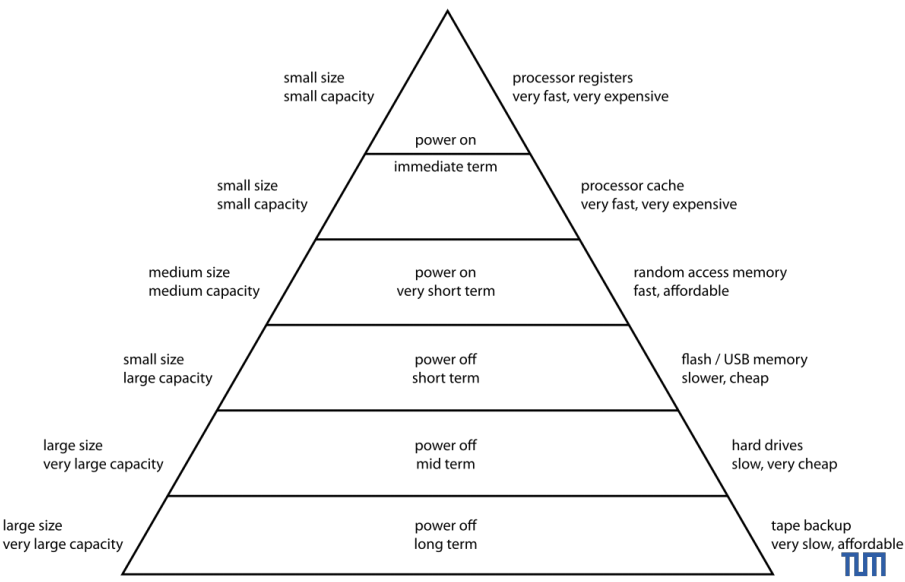
\includegraphics[width=0.8\textwidth]{storage.png}
\end{figure}
\subsubsection{Local Storage}

\paragraph{Redundant Array of Independent Disks -- RAID}
\begin{itemize}
	\item Goal: increase reliability or bandwidth
	\item RAID 0: \textbf{distribute} blocks over \textbf{2 disks}, if \textbf{write both blocks on two disks} at the same time, it gets \textbf{double bandwidth} to the disk.
	
	$\rightarrow$ \textbf{higher bandwidth}
	\item RAID 1: \textbf{replicates} blocks on \textbf{2 disks}. If one fails, we still have the information on the other disk. 
	
	$\rightarrow$ \textbf{higher reliability}
	\item RAID 5: \textbf{distribute} blocks over \textbf{4 disks}, while one disk saves the \textbf{parity information}. If one block fails, the parity information enables \textbf{reconstruction}. Parity information of blocks is not written on the same disk, but \textbf{distributed} over all disks.
	
	$\rightarrow$ \textbf{higher bandwidth and reliability}
\end{itemize}
\paragraph{Flash}
\begin{itemize}
	\item non-volatile memory, retains stored information even after power is removed.
	\item Write operation: tunnel injection, a high positive voltage between control gate and source \textbf{pushes electrons into the floating gate}. It stays/saves in the floating gate as stored information. 
	\item Read operation: a higher voltage is required at the drain to make the channel conduct, the electrons move from source to drain.
	\item Increasing storage density: \textbf{increase floating gates} in a flash cell
	\begin{itemize}
		\item Single Level Cells (SLC): stores \textbf{1 bit} of information
		\item Multiple Level Cells (MLC): stores \textbf{2 bits} of information
		\item \# floating gates $\uparrow$, cost per bit $\downarrow$, storage density $\uparrow$, program-erase cycles $\downarrow$, write/reading speed $\downarrow$
	\end{itemize}
	
	\item Use-case: USB-disks, SD-cards, mobile phone storage, built in SSD
\end{itemize}

\paragraph{SSD}
\begin{itemize}
	\item Comparison with hard disks:
	\begin{itemize}
		\item lower latency, random access
		\item smaller storage capacity
		\item less power hungry
		\item faster read/write speed
	\end{itemize}
\end{itemize}

\subsubsection{Data Center Storage}
\begin{itemize}
	\item storage comparison: \euro/IOPS 
	\item only based on flash storage or SSDs, combined with RAID, with special controllers optimized for SSDs.
	
	$\rightarrow$ IOPS $\uparrow$, latency $\downarrow$, bandwidth $\uparrow$, cost $\uparrow$
\end{itemize}


\subsubsection{Provisioning of Storage}
\begin{itemize}
	\item 3 ways to provide storage:
	\begin{itemize}
		\item Direct Attached Storage: storage devices are attached to the individual computer
		\item Storage Area Network
		\item Network Attached Storage
	\end{itemize}
\end{itemize}


\paragraph{Storage Area Network -- SAN}
\begin{itemize}
	\item access to \textbf{block level} data storage
	\item a \textbf{specialized network} connecting the servers which separates from LAN
	\item \textbf{no pre-existing file system}, the server can define its own file system according to needs
	\item a shared pool of spare resources, which allows \textbf{flexible allocation of spare storage} 
	
	\item Advantages:
	\begin{itemize}
		\item \textbf{flexible distribution} of devices between clients, reconfiguration of distribution in software instead of adaptation of cabling.
		\item easy replacement of faulty servers
		\item back-up can be done centrally, easier disaster protection
		\item no pre-existing file system, allows \textbf{customization} according to needs.
	\end{itemize}
	Disadvantages:
	\begin{itemize}
		\item shared network bandwidth
		\item shared performance of storage devices
	\end{itemize}
\end{itemize}
\begin{figure}[H]
	\centering
	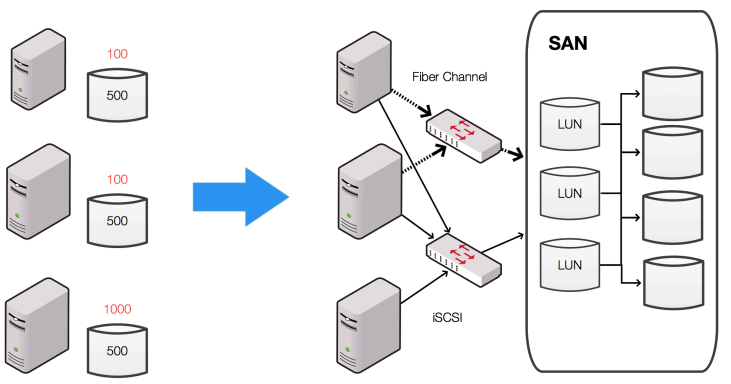
\includegraphics[width=0.7\textwidth]{san.png}
\end{figure}

\paragraph{Network Attached Storage -- NAS}
\begin{itemize}
	\item storage devices(disks) are connected to a \textbf{file server}
	\item computers \textbf{go over the network} and \textbf{access the file system} on file server
	\item an \textbf{existing file system}.
	\item network file sharing protocols: NFS
	\item storage devices: RAID to increase bandwidth and reliability
	\item Use-case: streaming contents(movies, images) to home network. If connected to home WiFi, then access to local storage. Access out of home using VPN and public IP
	
\end{itemize}
\begin{figure}[H]
	\centering
	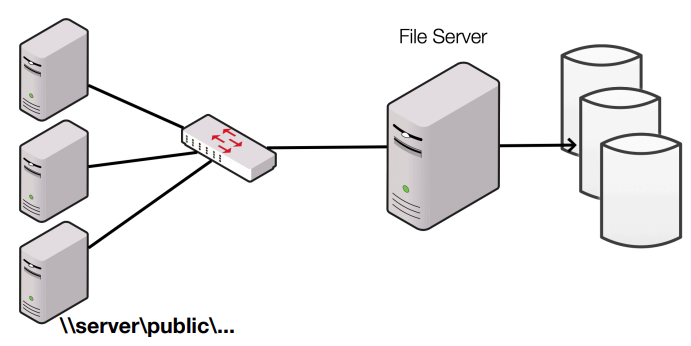
\includegraphics[width=0.7\textwidth]{nas.png}
\end{figure}


\subsubsection{Storage Virtualization}
\begin{itemize}
	\item Goal: location transparency
	\item Process: allocate a \textbf{virtual disk}, which will be \textbf{mapped to a real physical hard-disk} in the Storage Area Network. The \textbf{client won't know about which hard-disk is allocated} for the virtual disk.
\end{itemize}
\paragraph{Block Virtualization}
\begin{itemize}
	\item the \textbf{mapping} of a \textbf{virtual disk and block number} to a \textbf{physical disk and block number}.
	\item Use-case: SAN, flexible mapping, disk expansion and shrinking
	\item implementation:
	\begin{itemize}
		\item host based: host runs virtualization software
		\item storage device based: disk array provides a virtualization level
		\item \textbf{network based}: virtualization device is in LAN and connected to a SAN, \textbf{most frequent implementation}
		\begin{itemize}
			\item \textbf{in-band}: client sends request for certain blocks to the controller in the network, the controller fetches the data and returns the data to the client.
			\item \textbf{out-of-band}: host contacts the controller, gets the mapping information and accesses the data in SAN directly without the help of controller.
		\end{itemize}
	\end{itemize}
\end{itemize}

\paragraph{File Virtualization}
\begin{itemize}
	\item Virtualization on \textbf{file level}
	\item Use-case: \textbf{Distributed File System}
	\begin{itemize}
		\item allows transparent access to multiple NAS server. Files located on multiple NAS servers \textbf{appears as if on a single NAS}, the client doesn't know on which server the file exists.
	\end{itemize} 
\end{itemize}

	\section{Virtualization}
\begin{itemize}
	\item Idea: resource usage by a single user is \textbf{under-utilized}, the \textbf{efficiency} of usage of resource is \textbf{low}.
	
	$\rightarrow$ own a machine in a shared manner $\rightarrow$ \textbf{virtualization}
	\item Definition: Virtualization is a computer architecture technology where \textbf{multiple virtual machines} are \textbf{multiplexed} in the \textbf{same hardware}. (all VMs are connected and are owners of the hardware)
	\item Goal:
	\begin{itemize}
		\item enhance resource sharing, \textbf{improve} machine \textbf{efficiency}
		\item able to replace and upgrade hardware \textbf{on the fly}, \textbf{without interrupting the running program or rebooting}.
		\item reduce down time
		\item \textbf{faster provisioning} of multiple machines 
	\end{itemize}
	\item Modes of operation:
	\begin{itemize}
		\item \textbf{kernel mode}: higher privilege
		\begin{itemize}
			\item OS allows execution of \textbf{all CPU instructions}
			\item kernel codes \textbf{don't execute in user mode}.
			\item execute in \textbf{superuser/supervisor} privilege. 
		\end{itemize}
		
		\item \textbf{user mode}:
		\begin{itemize}
			\item OS allows execution of \textbf{few CPU instructions}
			\item if user applications have to execute \textbf{privileged instructions}, they \textbf{ask kernel} to execute. 
			\item execute in user privilege.
		\end{itemize}
	\end{itemize}
\end{itemize}

\subsection{Technology for Virtualization: Hypervisors}
A \textbf{hypervisor} (or virtual machine monitor, VMM) is a kind of emulator; 
it is computer software, firmware or hardware that \textbf{creates and runs virtual machines}. 
A \textbf{computer on which a hypervisor runs} one or more virtual machines is called a \textbf{host machine}, and \textbf{each virtual machine} is called a \textbf{guest machine}. 


The hypervisor \textbf{presents the guest operating systems with a virtual operating platform and manages the execution of the guest operating systems}. Multiple instances of a variety of operating systems may \textbf{share the virtualized hardware resources}: for example, Linux, Windows, and macOS instances can all run on a single physical x86 machine. 


This contrasts with operating-system-level virtualization, where all instances (usually called containers) must share a single kernel, though the guest operating systems can differ in user space, such as different Linux distributions with the same kernel.

\subsubsection{Bare-Metal Hypervisor}
\begin{itemize}
	\item runs \textbf{directly} on \textbf{host's hardware} -- Ring 0
	\item Guest OS operates at Ring 1
	\item provides \textbf{almost full isolation} to the users. All Guest OSs are \textbf{independent} and are owner of the hardware. VMM \textbf{controls the hardware and to manages resource allocation to guest OSs}.
	\item Use-case: Hyper-V, ESX, Xen
	
\end{itemize}

\subsubsection{Hosted Hypervisor}
\begin{itemize}
	\item \textbf{runs on a conventional OS} just as other computer programs
	\item abstracts guest OSs from the host OS. 
	\item Use-case: VMware player, VMware workstation, VirtualBox
\end{itemize}

\begin{figure}[H]
	\centering
	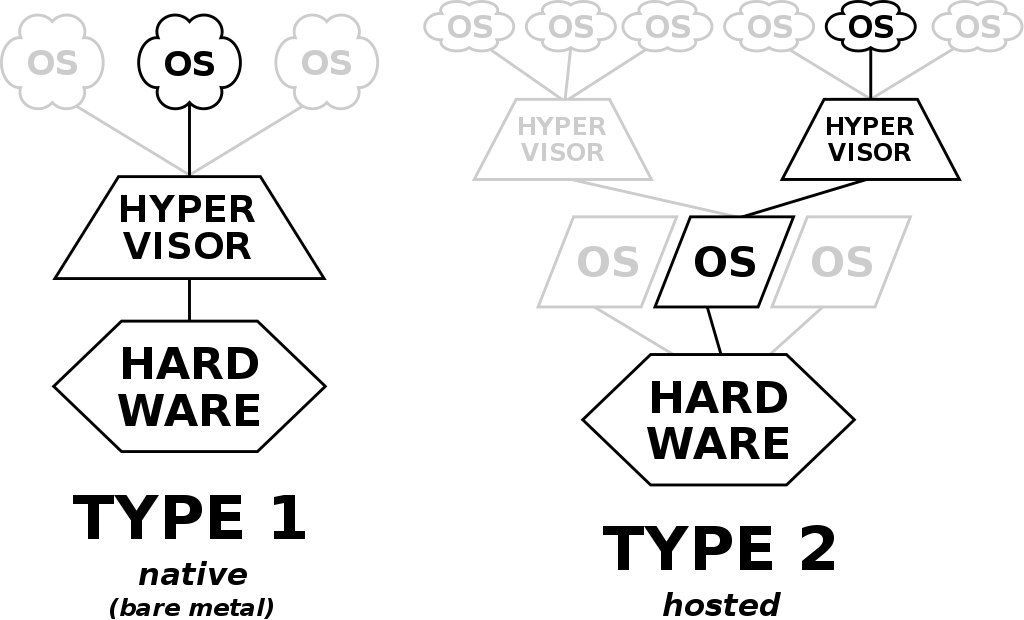
\includegraphics[width=0.65\textwidth]{hypervisor.png}
\end{figure}

\subsection{Full Virtualization}
\begin{itemize}
	\item for \textbf{any guest OS without any modifications} 
	\item VMM works in Ring 0, guest OSs work in Ring 1  -- Bare-metal hypervisor
	\item Problem: \textbf{execution error} of privilege instructions from guest OS being in \textbf{lower ring} (Ring 1)
	\begin{itemize}
		\item Solution: VMM intercepts such error and \textbf{emulates} the instructions \textbf{on the fly}
		
		$\rightarrow$ not all instructions are trapped.
		
		\item Solution: a \textbf{binary translator}, which overrides these privileged instructions and places them in translation cache. 
	\end{itemize}
	\item Consequences:
	\begin{itemize}
		\item system calls: takes \textbf{10 times more cycles} compared to no hypervisor, because \textbf{fault message} are issued, translated and executed \textbf{for every system call}. 
		
		\item I/O virtualization: major issue. \textbf{more I/Os} due to more CPUs (guest computers) but I/O chipset \textbf{can't be easily extended}
		
		
		\item memory virtualization: 2-stage mapping process with VMM.
		\begin{itemize}
			\item program's memory addresses $\rightarrow$ virtual physical memory (on VMM) $\rightarrow$ real physical memory
			\item VMM maintains a \textbf{shadow page table}, this process takes \textbf{3 to 400 more cycles} than without VMM.
		\end{itemize}
		
		
	\end{itemize}
	

\end{itemize}

\subsection{Paravirtualization}
\begin{itemize}
	\item guest OS needs to be \textbf{modified at source code level}. Information is given in prior in code, that if such instruction is being executed, it needs to go directly to the VMM instead of the hardware. 
	
	$\rightarrow$ no execution error because of ring privilege. $\rightarrow$ no trapping or binary translation needed 
	
	\item Hypervisor provides \textbf{interface} to accommodate critical kernel operations (memory management, interrupt handling)
	\item Advantages:
	\begin{itemize}
		\item runtime changes are avoided. (no on-the-fly modification)
		\item unnecessary trapping of critical instruction avoided (modified in code)
		\item lower virtualization overhead
	\end{itemize}
	Disadvantages:
	\begin{itemize}
		\item a modified guest OS needed when changing machines.
	\end{itemize}
	
\end{itemize}

\subsection{Hardware-assisted Virtualization}
\begin{itemize}
	\item Idea: enables efficient full virtualization using \textbf{help from hardware capabilities}, primarily from the host processors. 
	
	$\rightarrow$ a processor extension is introduced in a \textbf{higher priority layer} -- Root mode privilege level with VMM.
	
	\item Guest OS now operates at \textbf{Ring 0} and can execute all critical instructions
\end{itemize}

\begin{figure}[H]
	\centering
	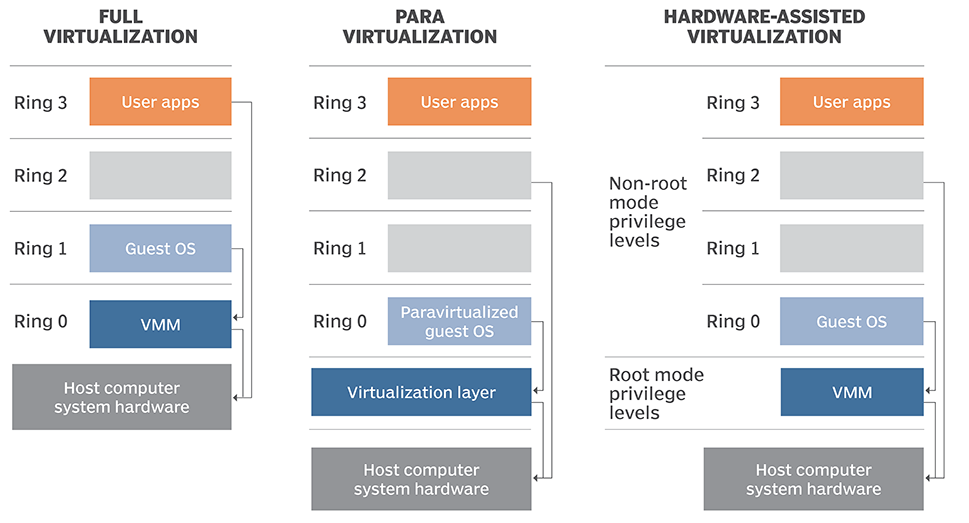
\includegraphics[width=0.7\textwidth]{virtualization.png}
\end{figure}

\subsection{OS-Level Virtualization}
\begin{itemize}
	\item Idea: 
	\begin{itemize}
		\item disadvantages of hypervisor-based virtualization: OS dependent, not scalable, not portable, slow deployment. 
		\item higher scalability required in application.  
	\end{itemize}
	$\rightarrow$ \textbf{OS-Level virtualization}
	\item VMM is \textbf{on top of host OS}
	\item building blocks: linux kernel features
	\begin{itemize}
		\item \textbf{namespaces}: \textbf{limit the views}, wrap a group of resources for limited access, managed using APIs
		\begin{itemize}
			\item PID: create another set of PID
			\item cgroup: new views to root directories
			\item network: new views to network resources
		\end{itemize}
		\item \textbf{cgroups}: control groups, \textbf{limits the applications to a specific set of resources}
		\begin{itemize}
			\item memory cgroup: memory resource controller, isolates the memory behavior of a group of task from others. when memory exceeds, running processes will be killed.
			\item others: cpu, blkio, cpuset, devices, freezer cgroup
		\end{itemize}
		
	\end{itemize}
	\item \textbf{Container}: 
	\begin{itemize}
		\item allows multiple \textbf{isolated} linux systems of same kind on a single host OS.
		\item resources are \textbf{isolated in a container} for each user.
		\item it utilizes \textbf{cgroups and namespaces} to limit the views and resources of each container.
		\item Use-case: \textbf{Docker}
		\item Advantages:
		\begin{itemize}
			\item runtime isolation: isolates different runtime environments based on application requirement
			\item cost-efficiency: no creation of entire virtual OS for each user.
			\item easy portability of containers
			\item high scalability, easy replication of containers across environments
			\item faster deployment: layer-concept, only new layers/updated layers are built. 
			 
		\end{itemize}
	\end{itemize}
	\begin{figure}[H]
		\centering
		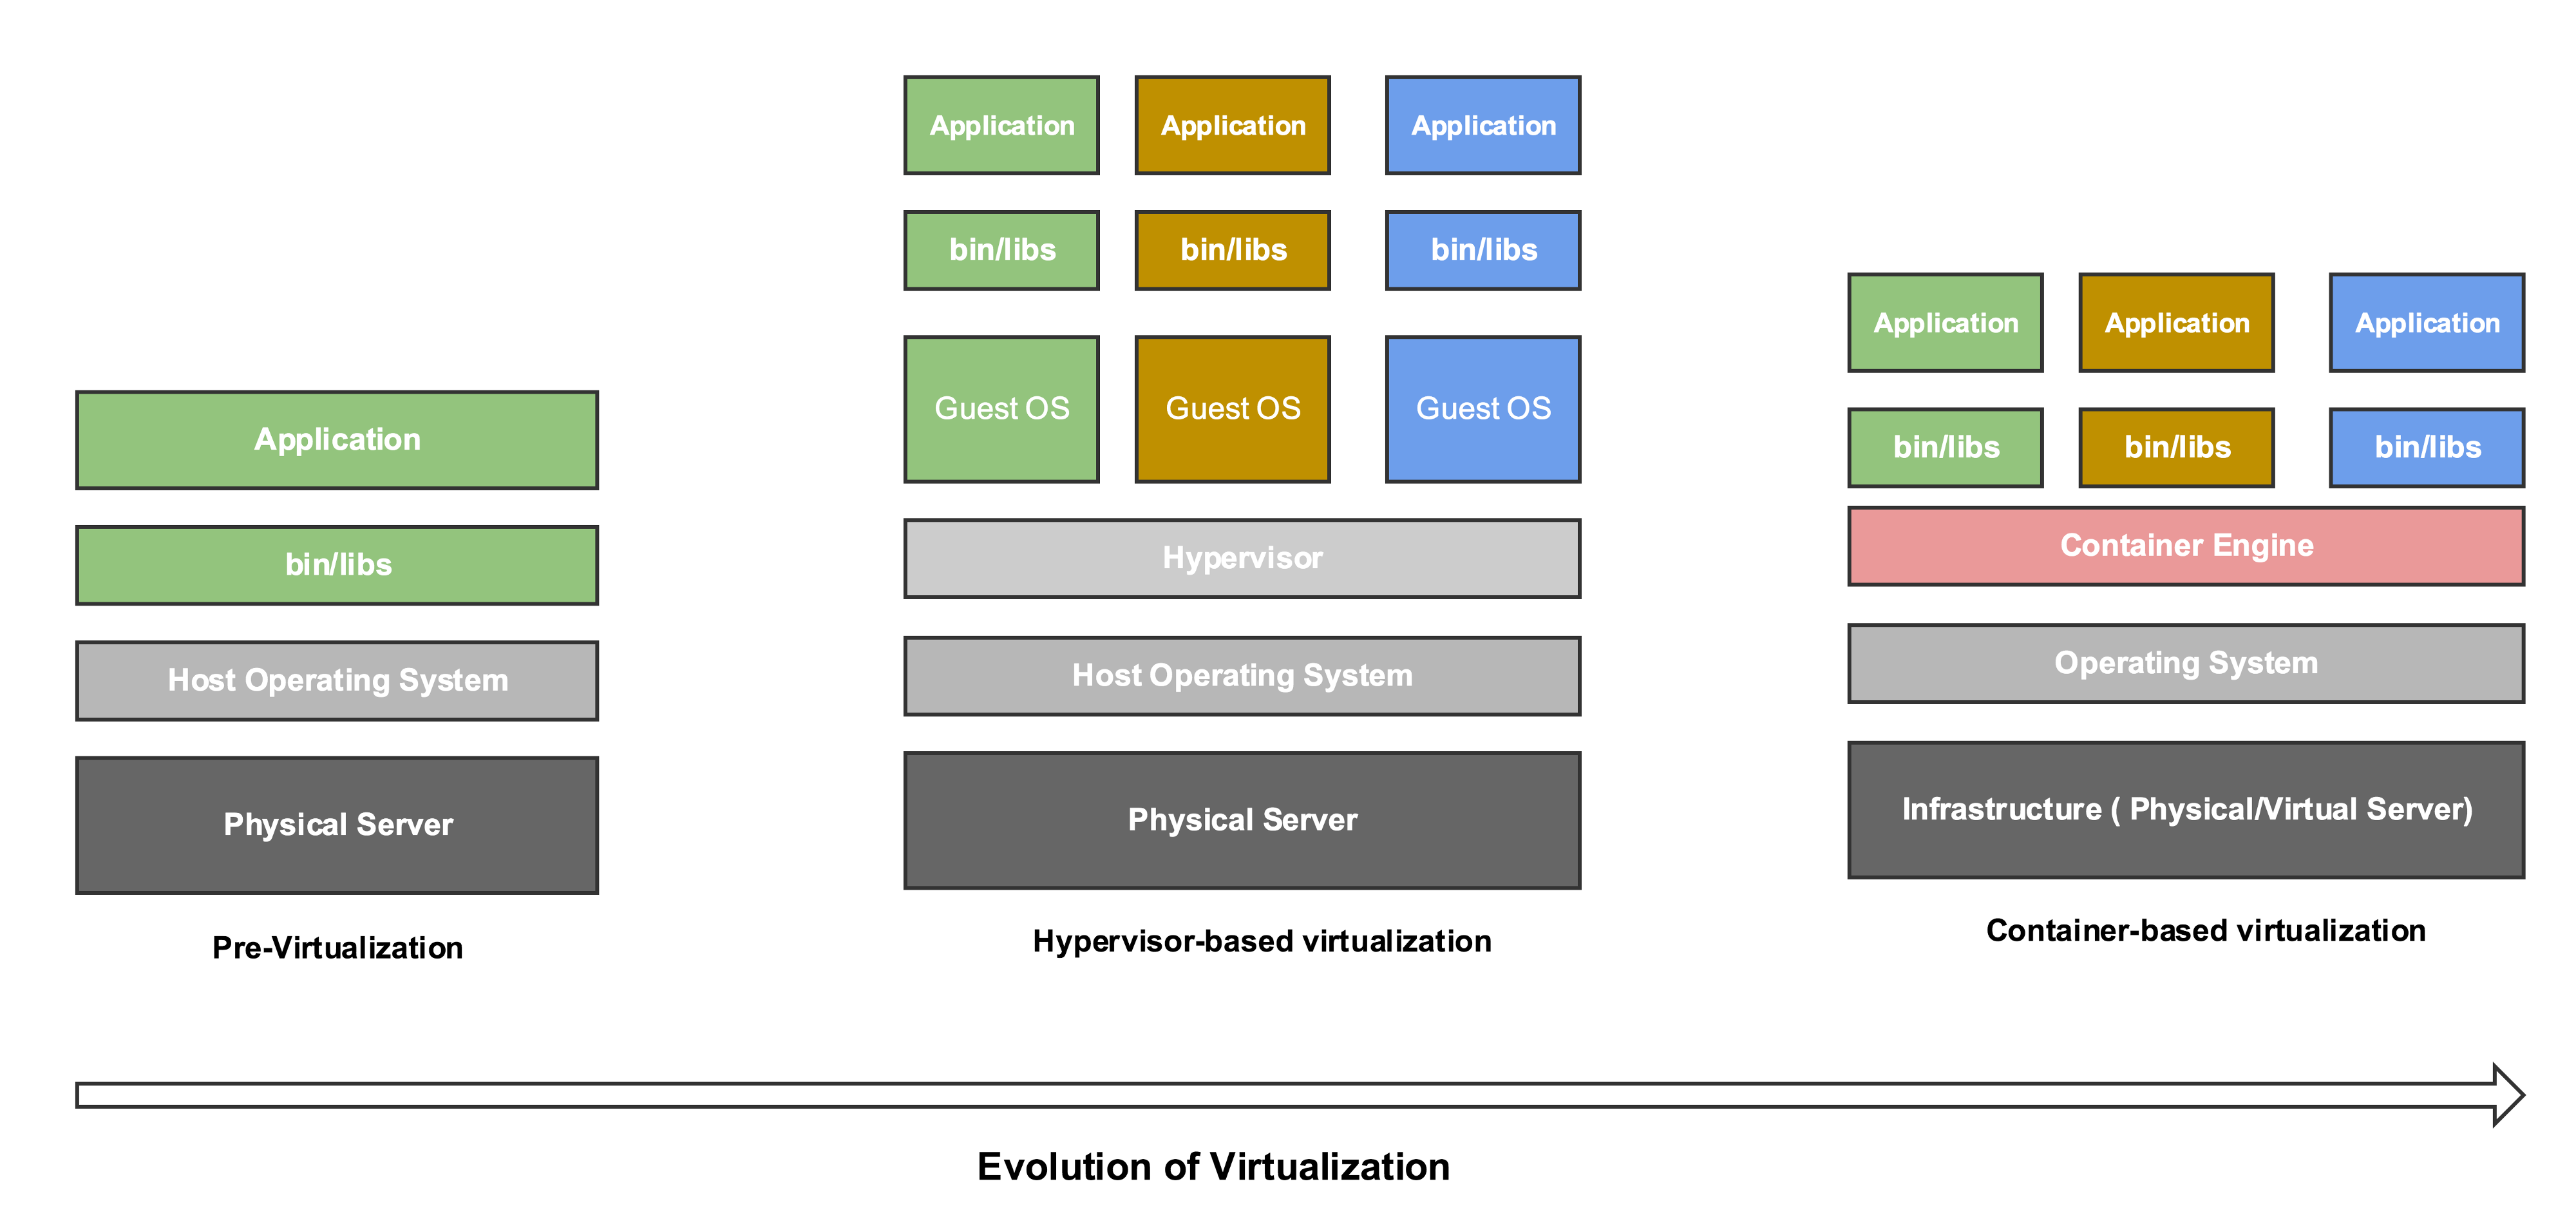
\includegraphics[width=\textwidth]{container.png}
	\end{figure}
\end{itemize}


	\section{Infrastructure as a Service -- Amazon Web Service}

AWS is distributed among \textbf{regions}. Each region is \textbf{isolated} for \textbf{fault tolerance and stability}. Each region consists of \textbf{availability zones} (eg: data centers), where data can be \textbf{replicated}. 

\begin{itemize}
	\item region availability: 99.99\% from Amazon's SLA(service level agreement). To profit from SLA, data must be replicated over at least 2 zones in case of failure.
	\item IaaS service model:
	\begin{itemize}
		\item compute: EC2,
		\item network: VPC, CloudFront
		\item storage: S3, EFS, EBS, instance storage
	\end{itemize}
\end{itemize}

\subsection{Compute Service: Elastic Compute Cloud EC2}
\begin{itemize}
	\item \textbf{virtual machine instance} running based on an AMI
	\item \textbf{Amazon Machine Image}: a copy of server with OS and preinstalled software (eg: Ubuntu server 18.04 LTS, SSD volume type)
	\item instance attached \textbf{ephemeral storage, block storage and virtual firewall}
	\item resource allocation through Xen Hypervisor (\textbf{bare metal hypervisor}) 
	\item \textbf{elastic IP address} possible: private \& public IP address \textbf{remains same} after start/stop 
	\item lifecycle: pending -- running -- stopping -- stopped --shutting down -- terminated
\end{itemize}

Comparison Amazon EBS-Backed \& Instance Store-Backed EC2 instance:

\begin{table}[H]
	\begin{center}
	\begin{tabular}{|l|p{5cm}|p{5cm}|}
		\hline
		Characteristics  &EBS-Backed  & Instance Store-Backed \\ \hline
		root device volume        &EBS volume  & Instance store volume   \\ \hline
		stopped state     & stop-state exists, restart at a different server possible  & no stop-state, only termination    \\ \hline
		data persistence       & lost when termination, kept in EBS when stopped  & lost when termination   \\ \hline
		modification  & modifiable at stop-state  & fixed    \\ \hline
	\end{tabular}
\end{center}
\end{table}

\subsection{Storage}
\begin{itemize}
	\item \textbf{Elastic Block Storage (EBS)}
	\begin{itemize}
		\item similar to Storage Area Network (SAN)
		\item can be \textbf{mounted into VM}
		\item multiple block storage can be \textbf{combined into RAID}
		\item \textbf{snapshots} of the block storage are \textbf{stored in S3 for backup or replication}
	\end{itemize}
	\item \textbf{EC2 instance storage}: 
	\begin{itemize}
		\item disk or SSD connected to the physical machine
		\item \textbf{data erased} when instance is \textbf{stopped or terminated}
	\end{itemize}
	\item \textbf{Elastic File System (EFS)}: 
	\begin{itemize}
		\item similar to Network Attached Storage (NAS), scalable
		\item can be created and mounted into VM
		\item files can be \textbf{shared among instances}
	\end{itemize}
	\item \textbf{Simple Storage Service (S3)}
	\begin{itemize}
		\item large size storage (up to 5TB)
		\item \textbf{slower access} compared to EBS or local disks, \textbf{high durability, low availability}
		\item Use-case: backup
	\end{itemize}
\end{itemize}

\begin{figure}[H]
	\centering
	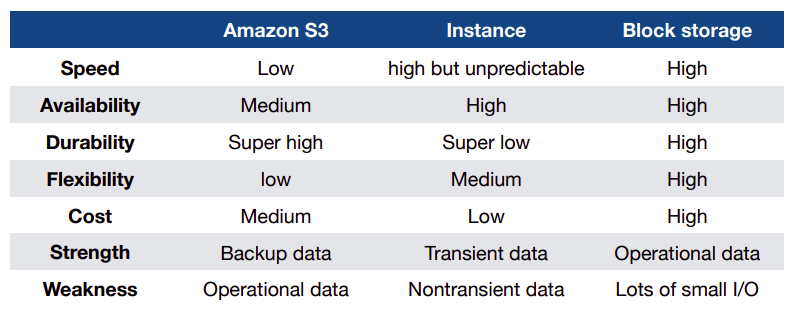
\includegraphics[width=0.8\textwidth]{awsstorage.png}
\end{figure}

Storage attached to EC2:
\begin{itemize}
	\item root device volume: EBS, instance storage. 
	\begin{itemize}
		\item instance stops: data \textbf{preserved}
		\item instance terminates: data \textbf{deleted}
	\end{itemize}
	\item instance store volume: local disks of the server. Data \textbf{erased} if instance stops
	\begin{itemize}
		\item instance stops: data \textbf{erased}
		\item instance terminates: data \textbf{erased}
	\end{itemize}
\end{itemize}

\subsection{Network}
\begin{itemize}
	\item \textbf{elastic IP address}: public IP address \textbf{remains same} even after start/stop.
	\item \textbf{Virtual Private Cloud (VPC)}: 
	\begin{itemize}
		\item resembles network in own data center, resources are launched into own VPC
		\item configuration of IP address range, subnets, route tables, network gateways, firewall settings	
	\end{itemize}
	\item \textbf{CloudFront}: content distributed network
	\begin{itemize}
		\item automatic distribution: content changes in S3 and will be automatically updated in every data center from edge locations
		\item response delivered from data center closed to requester.
	\end{itemize}
\end{itemize}


\section{Cloud Storage Systems}
\begin{itemize}
	\item Comparison VM storage VS. Cloud storage:
	\begin{itemize}
		\item VM: instance volume -- lost when VM stops, EBS volume -- lost when VM terminates.
		\item Cloud storage: for voluminous data potentially long-term storage.
	\end{itemize}
	\item requirements:
	\begin{itemize}
		\item voluminous data
		\item commodity hardware
		\item distributed data
		\item failures is norm rather exception: replication \& fault tolerance
		\item processed by application
		\item optimized for typical access patterns
	\end{itemize}
	\item \textbf{CAP Theorem}: aim for \textbf{availability} or \textbf{consistency}. Partition-tolerance has to be guaranteed.
	\item Types:
	\begin{itemize}
		\item object storage: S3
		\item shared file systems: NAS, EFS
		\item relational databases
		\item noSQL databases
		\item Data warehouse
	\end{itemize}
\end{itemize}

\subsection{Object Storage: AWS S3}
\begin{itemize}
	\item Goal: infinite data \textbf{durability} by 99.99\% availability
	\item Use-case: short-term or long-term \textbf{backup}
	\item storage classes:
	\begin{itemize}
		\item standard: for \textbf{frequently accessed} data
		\item reduce redundancy: for \textbf{reproducible, infrequently accessed} data
		\item intelligent tiering: objects are \textbf{automatically moved} between frequent and infrequent access tier.
		\item glacier: long-term data archive. long retrieval time
		\item deep-archive: even longer retrieval time, for \textbf{rarely accessed} data.
	\end{itemize}
	\item Data access: objects can be uploaded, retrieved and deleted. \textbf{No modification}.
	\item Versioning: versioning for individual files or entire buckets.
	\item Lifecycle: consists of rule that triggers \textbf{transition} to other storage classes or \textbf{expiration} of objects.
	\item consistency: \textbf{eventual consistency}. simultaneous puts -- last write wins.
\end{itemize}


\subsection{File Storage: Google File System}

\begin{itemize}
	\item \textbf{distributed} file system
	\item architecture:
	\begin{itemize}
		\item 1 \textbf{master server} + many \textbf{chunk servers}
		\item \textbf{master server}: metadata in main memory stored as \textbf{lookup table}
		\item \textbf{chunk server}: stores many 64MB-chunks as linux files.
		\item shadow masters possible to reduce load on master server
		\item \textbf{decoupled} control and data flow. \textbf{Control flow runs through master server} to chunk server, \textbf{data can directly flow from chunk server to client}.
	\end{itemize}
	\item replication: data is replicated to balance workload and combat failures.
	\item data access: client \textbf{first contacts master server} and finds out the corresponding chunk server through lookup table. Later interactions(writes, read) \textbf{directly between chunk and client}. 
	\item consistency: cocurrent writes possible, but only writes on \textbf{primary chunk} will be \textbf{replicated}. \textbf{consistent but undefined state}.
	\item Limitations:
	\begin{itemize}
		\item scalability of single master $\rightarrow$ development of distributed master
		\item fixed chunk size, while application can have smaller files.
		\item no latency guarantees.
	\end{itemize}
	\item other file systems: AWS Elastic File System
\end{itemize}

\subsection{Relational Database}

\begin{itemize}
	\item data represented as \textbf{n-ary relations}. Each relation is a \textbf{table}, which is defined by \textbf{schema}.
	\item data access: SQL-queries
	\item \textbf{ACID-properties} of transactions: atomicity, consistency, isolation, durability
	\item designed for \textbf{vertical scaling}
	\item Installation of own database:
	\begin{itemize}
		\item installation and management \textbf{on you own}
		\item data management: certificate, patching, performance tuning, backup, scaling, security 
	\end{itemize}
	\item Cloud relational database service: Amazon \textbf{managed} RDS, Amazon Aurora (own relational database)
	\begin{itemize}
		\item \textbf{managed} standard relational databases: mySQL, PostgreSQL
		\item different \textbf{certifications provided}
		\item \textbf{pre-configured} database instances
		\item standby copies in case of failovers
		\item multiple read replicas to increase read throughput, guarantee fault tolerance
		\item \textbf{automatic} backup snapshots in S3, \textbf{automatic} scaling
	\end{itemize}
\end{itemize}

\subsection{NoSQL Database}

\begin{itemize}
	\item database for \textbf{non-relational} data \textbf{without predefined schema}. Easy to define new attributes.
	\item designed for \textbf{horizontal scaling}
	\item Types of NoSQL databases:
	\begin{itemize}
		\item key-value database: Amazon Dynamo
		\item document oriented
		\item graph database
	\end{itemize}
	\item Cloud NoSQL database service: Amazon Dynamo DB
	\begin{itemize}
		\item \textbf{distributed} data store $\rightarrow$ optimized for \textbf{small} request, \textbf{quick} access and \textbf{high availability}.
		\item \textbf{key-value} database
		\begin{itemize}
			\item \textbf{primary key}: unique for each row, \textbf{composite key} possible (partition key + sort key).
			\item values: a set of attributes
		\end{itemize}
		\item Architecture:
		\begin{itemize}
			\item \textbf{key-value pairs} stored in \textbf{tables}. 
			\item \textbf{tables} stored in \textbf{partitions}
			\item number of partitions depends on: size, required read/write capacity units
		\end{itemize}
		\item management of partitions: key $\rightarrow$ partition $\rightarrow$ virtual node $\rightarrow$ physical nodes
		\begin{itemize}
			\item key $\rightarrow$ partition: key-value pair entries are \textbf{hashed by keys} onto a \textbf{ring space} of partitions.
			\item partition $\rightarrow$ node: \textbf{ring} is split into \textbf{segments containing multiple partitions}. Each segment is managed by a \textbf{virtual node}.
			\item virtual node $\rightarrow$ physical node
		\end{itemize}
		\item Replication: (N, R, W)
		\begin{itemize}
			\item N: replication to \textbf{N consecutive nodes}. N $\uparrow$, durability $\uparrow$
			\item R: success \textbf{read} on \textbf{R copies}. R $\downarrow$, latency $\uparrow$
			\item W: success \textbf{write} on \textbf{W copies}. W $\downarrow$, latency $\uparrow$
			\item \textbf{R + W > N}: ensures the \textbf{most recent write} is returned.
		\end{itemize}
		\item Consistency: \textbf{eventual consistency}
		\item Failures is a \textbf{norm}: \textbf{gossip protocol}
		

	\end{itemize} 
\end{itemize}


	\section{Infrastructure as a Service -- OpenStack}
\begin{itemize}
	\item main services:
	\begin{itemize}
		\item Compute: Nova, central computation
		\item Identity: Keystone, \textbf{authentication}, generate \textbf{token} for subsequent calls
		\item Image: Glance, base image selection for VM (\textbf{template for VM})
		\item Networking: Neutron, determine networking \textbf{rules}, allocate \textbf{network resources}
		\item Dashboard: Horizon
		\item Block storage: Cinder, allocate \textbf{volume}
	\end{itemize}
	\item Design concepts:
	\begin{itemize}
		\item Goal: scalability (horizontal), elasticity
		\item \textbf{asynchronous} communication: message \textbf{queues}
		\item \textbf{decentralized} data management: each microservice has its \textbf{own database}, accepts \textbf{eventual consistency}
		\item \textbf{distribute} everything: distributed into microservices, communication through APIs
	\end{itemize}
	\item Architecture:
	\begin{figure}[H]
		\centering
		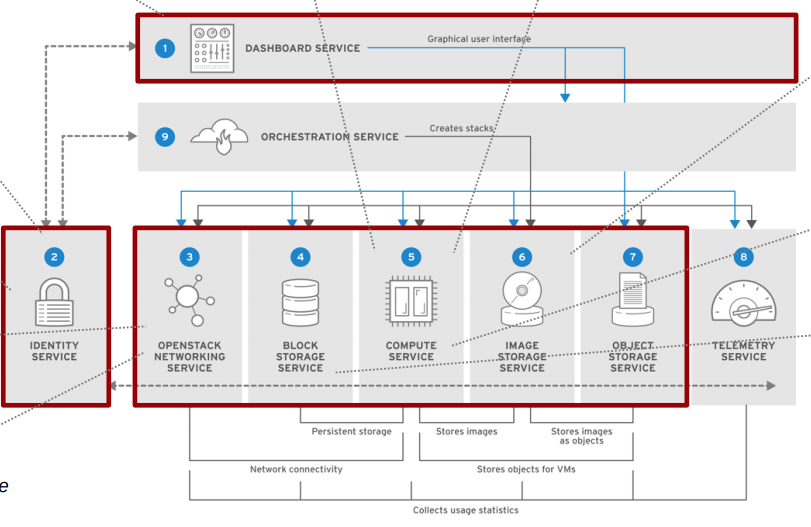
\includegraphics[width=\textwidth]{openstack.png}
	\end{figure}
\end{itemize}

\subsection{Identity Management}
\begin{itemize}
	\item provides authentication credential validation and data
	\item generates \textbf{authentication tokens} that enable clients to access OpenStack services REST APIs.
	\item clients obtain this \textbf{token} and \textbf{URL endpoints} for other service APIs.
\end{itemize}

\subsection{Compute Service}
\begin{itemize}
	\item manage and provision \textbf{virtualized server resources}: CPU/memory/disk/network
	\item VM management: start/stop/reboot/terminate
	\item communication with other services: image, identity, network, storage services
	
\end{itemize}

\paragraph{components:}
\begin{itemize}
	\item Nova API: interface to create instances
	\item RabbitMQ and compute database : provides communications hub and manage data persistence
	\begin{itemize}
		\item Message \textbf{Queue}(MQ): pass messages between services \textbf{asynchronously}
		\item compute database: \textbf{store} build-time and run-time \textbf{states}, available instance types/in use, available networks etc.
	\end{itemize}
	\item Scheduler: determines \textbf{allocation of physical hardware} to virtual resource using \textbf{series of filters}
	\item \textbf{compute node}: \textbf{management of all interactions} with individual endpoints providing computing resource
\end{itemize}

\subsection{Network, Block Storage and Image Storage}
\begin{itemize}
	\item network: manage \textbf{networks, ports, attachments on infrastructure} for virtual resources
	\item block storage: 
	\begin{itemize}
		\item create and manage \textbf{lifecycle of volumes}
		\item respond to \textbf{read and write requests} sent to block storage to maintain states
		\item \textbf{backup} volumes
	\end{itemize}
	\item image storage:
	\begin{itemize}
		\item storage in \textbf{independent} image \textbf{database}	
		\item accept API calls for \textbf{image discovery, retrieval and storage}
	\end{itemize}
	
\end{itemize}


\subsection{Server Creation Workflow}
\begin{itemize}
	\item Nova Client gets \textbf{token} from Identity Management service.
	\item After \textbf{authentication}, Nova API \textbf{sends request} of launching instance \textbf{into Message Queue}
	\item Nova scheduler \textbf{subscribes request} and \textbf{allocate resources using filtering}
	\item Nova compute communicates with Image service, Network service, block storage service to \textbf{get image, allocate network and storage}.
	\item Nova compute starts instance.
\end{itemize}


\section{Infrastructure as a Service -- Microsoft Azure}
\begin{itemize}
	\item \textbf{company-oriented} service
	\item services:
	\begin{itemize}
		\item Azure Virtual Machines
		\item Azure Virtual Network: connects \textbf{VMs and services}, connect \textbf{cloud resources with on-premise resources} through \textbf{Internet} via VPN.
		\item Azure ExpressRoute: connects \textbf{cloud resources and on-premise resources} via \textbf{dedicated lines}.
	\end{itemize}
	\item \textbf{Traffic Manager}: distribute resources to either Azure or on-premise data centers -- different service endpoints.
	\item \textbf{Resource Manager}: management as a \textbf{group}. Resource allocation defined in \textbf{template} with version control. 
\end{itemize}
	\part{Platform as a Service -- PaaS}
\begin{itemize}
	\item Definition: 
	\begin{itemize}
		\item client: deploy \textbf{customer-created applications}
		\item cloud provider: provides web interfaces, programming languages, libraries, services and tools 
	\end{itemize}
	\item Rights as customer:
	\begin{itemize}
		\item application deployment
		\item configuration settings application-hosting environment
	\end{itemize}
	\item No control:
	\begin{itemize}
		\item cloud infrastructure: storage, network, servers, operation systems
	\end{itemize}
\end{itemize}

\section{Platform as a Service -- Microsoft Azure}
\begin{itemize}
	\item Focus: integration with \textbf{on-premise IT} -- company oriented
	\item Services:
	\begin{itemize}
		\item Azure Web Apps
		\item Azure Service Fabrics: microservices
		\item Azure Functions
	\end{itemize}
	\item Azure access:
	\begin{itemize}
		\item \textbf{Tenant}: a Microsoft Active \textbf{Directory} for managing accounts, groups and permissions. (eg: a company)
		\item \textbf{Subscription}: a subscription is \textbf{associated with a unique tenant}. A \textbf{resource container} for the tenant.
		\begin{itemize}
			\item can be divided into \textbf{multiple resource groups}. (eg: different teams) Each has its \textbf{own resource allocation}.
			\item account (eg: an employee): has a \textbf{role} in subscription: eg: account administrator, service administrator 
		\end{itemize}
	\end{itemize}
\end{itemize}

\subsection{Azure Web Apps Service}
\begin{itemize}
	\item \textbf{development, deployment and management of web applications} without managing VMs
	\begin{itemize}
		\item different programming languages provided: development
		\item a \textbf{managed web environment}: deployment
		\item automatic load balancing: \textbf{scale in/out}
		\item VM sharing possible
	\end{itemize}
	\item App development:
	\begin{itemize}
		\item creation of a \textbf{deployment user}
		\item creation of a \textbf{resource group}: name, location, template
		\item creation of a \textbf{app service plan}: VM instance type, number of VM instances, scale count, subscription (resources), region, pricing tier.
		\item creation of a web app $\rightarrow$ development ready
	\end{itemize}
	\item App scaling: triggered by \textbf{automatic load balancing}, scales \textbf{according to app service plan}, apps will be \textbf{scaled together}. 
	\begin{itemize}
		\item manual scaling
		\item \textbf{automatic} scaling: according to defined metric/target/time period. 
	\end{itemize}
	\item App monitoring: 
	\begin{itemize}
		\item per app: 
		
		\begin{table}[H]
			\begin{center}
				\begin{tabular}{|l|p{7cm}|}
					\hline
					metrics  &definition \\ \hline
					Average response time        & time taken to serve requests (s)  \\ \hline
					Average memory working set     & average amount of memory used (MiB)    \\ \hline
					CPU time      & amount of CPU consumed (s)    \\ \hline
					Data In  & amount of incoming bandwidth (MiB)    \\ \hline
					Data Out  & amount of outgoing bandwidth (MiB)    \\ \hline
					Requests  & total number of requests regardless of HTTP status code    \\ \hline
				\end{tabular}
			\end{center}
		\end{table}
		
		\item per app service plan:
		\begin{table}[H]
			\begin{center}
				\begin{tabular}{|l|p{9cm}|}
					\hline
					metrics  &definition \\ \hline
					CPU percentage        & \textbf{average} CPU used \textbf{across all instances} (s)  \\ \hline
					memory percentage     & \textbf{average} memory used \textbf{across all instances} (MiB)    \\ \hline
					Data In  & \textbf{average} amount of incoming bandwidth \textbf{across all instances} (MiB)    \\ \hline
					Data Out  & \textbf{average} amount of outgoing bandwidth \textbf{across all instances} (MiB)    \\ \hline
					Disk Queue Length  & \textbf{average} amount of read \& write requests queued on storage (disk I/O)    \\ \hline
					HTTP Queue Length  & \textbf{average} amount of http-requests (plan load) \\ \hline
				\end{tabular}
			\end{center}
		\end{table}
		\item granularity (level of detail of data): minute/hour/day granularity metrics
	\end{itemize}
\end{itemize}


\subsection{Microservices Platform -- Azure Service Fabric}

\subsubsection{Monolithic VS. Microservices}
\begin{itemize}
	\item \textbf{Monolithic} service:
	\begin{itemize}
		\item tiered architecture (eg: presentation/user interface -- logic -- data layer)
		\item \textbf{replication} of the \textbf{whole app} to other instances
		\item all states stored in a single database.
		\item testing and failure: one part fails, the whole app fails. Changes of one part requires testing/deployment of whole app.
	\end{itemize}
	\item \textbf{Microservice}: 
	\begin{itemize}
		\item app is \textbf{decomposed} into microservices. 
		\item \textbf{individual replication} of each microservice over instances. \textbf{individual scaling}. 
		\item stateless services: \textbf{individual database} connected to microservice for state storage.
		\item stateful services: state is stored in the service. 
		\item testing and failure: \textbf{individual} testing and deployment. If one microservice fails, the rest is unaffected.
		\item increased network traffic and latency sensitivity: communication between microservices, especially chatty services.
	\end{itemize}
\end{itemize}

\subsubsection{Service Fabric}
\begin{itemize}
	\item platform for \textbf{microservice based applications}
	\item Transformation of a monolithic service to a microservice:
	\begin{itemize}
		\item lift and shift: containerize existing codes in service fabric
		\item modernization: add new microservices alongside the containerized codes
		\item innovate: break the monolithic service into microservices based on needs.
	\end{itemize} 
	\item Fabric cluster: \textbf{a set of virtual/real machines (nodes)} where microservices are deployed.
	\begin{itemize}
		\item service - node allocation: placement constraints of services, properties specified by node in key-value pairs.
		\item load balancing: \textbf{distributes/migrates} services to other nodes, \textbf{distributes requests}
		\item scaling of a whole cluster possible: app scaling
	\end{itemize}
	\item service models:
	\begin{itemize}
		\item reliable services model
		\item reliable actors model: \textbf{stateful} objects, actor \textbf{communicates} by receiving and sending \textbf{messages}.actor reacts faster than stateless services.
		\item guest executables: treated like stateless services
	\end{itemize}
	\item \textbf{service partition}: a group of service instances 
	\begin{itemize}
		\item stateless service: \textbf{not partitioned}. all instances belong to a \textbf{single partition}. eg: collection, gallery, overview
		\item stateful service: \textbf{frequently partitioned or replicated}. eg: by country, name, payment status  
	\end{itemize}
	\item testing:
	\begin{itemize}
		\item restart nodes/partitions of service instances
		\item simulate load balancing, failover, app-upgrade
		\item invoke data loss
		\item simulate scenarios: chaos(continuous overlapping faults), failover(continuous overlapping faults targeting single partition)
	\end{itemize}
\end{itemize}
	\section{Microservices Application Architecture}

\subsection{Monolithic Application Architecture}
\begin{itemize}
	\item a software program composing of \textbf{all in one piece}.
	\item each component is tightly \textbf{coupled}
	\item data: a single database
	\item layered/tiered architecture: 
	\begin{itemize}
		\item client-side user interface/presentation
		\item server-side application: performs detailed processing
		\item database
	\end{itemize}
	\item Advantages:
	\begin{itemize}
		\item easy development
		\item simple testing: end-to-end testing
		\item simple deployment
		\item easy horizontal scaling: run multiple copies of complete app behind a load balancer
	\end{itemize}
	Disadvantages:
	\begin{itemize}
		\item limitation in size and complexity: no continuous addition of codes
		\item large and complex size
		\item slow start time: dependent of size of application
		\item redeployment of \textbf{complete} app on minor updates
		\item low reliability: one module fails, the whole app fails.
		\item difficult to scale
	\end{itemize}
\end{itemize}

\subsection{Service Oriented Architecture}
\begin{itemize}
	\item functions of application as \textbf{service interfaces}
	\item data: a single database, data is \textbf{internally componentized}
	\item communication: each function logic \textbf{only accesses its data associated}. When \textbf{another function} requires data from other component, \textbf{communicate through interfaces}. 
\end{itemize}

\subsection{Microservices Architecture}
\begin{itemize}
	\item size: \textbf{split} the whole application into \textbf{a set of smaller and interconnected services}
	
	\item data: each service has \textbf{individual database/storage system}
	\item deployment: 
	\begin{itemize}
		\item each service runs \textbf{individually} on single or multiple machines.
		\item services communicates with common communication protocol (eg: REST).
	\end{itemize}
	\item operation: \textbf{stateless}, information is supplied on request. Once request is complete it's forgotten. 
	
	$\rightarrow$ allows rapid scaling
	
	\item Advantages:
	\begin{itemize}
		\item easier understanding and maintenance
		\item service independence: developed, tested and deployed independently
		\item fault resilience: one service fails, the rest is unaffected
		\item individual service scaling
	\end{itemize}
	Disadvantages:
	\begin{itemize}
		\item complexity of creating a distributed system: difficult testing, inter-process communication implementation necessary
		\item deployment complexity: each service instance needs to be configured, deployed, scaled and monitored. a \textbf{service discovery mechanism} implementation necessary.
	\end{itemize}

\end{itemize}

\subsection{Microservice Application Framework Components}
\subsubsection{API Gateway}
\begin{itemize}
	\item Idea: 
	\begin{itemize}
		\item monolithic: access to application through \textbf{single REST call}
		\item microservices: access to each microservice using different endpoints is suboptimal (client needs mismatch, difficult to refactor, in reality many microservices).
		
		$\rightarrow$ \textbf{API-Gateway}: a \textbf{single-entry point} into the system.	
	\end{itemize}
	\item encapsulates the whole internal system architecture. Clients don't know which microservice APIs are led to. 
	\item \textbf{separate} API-Gateways tailored for client(web, mobile, public): customize data sent back to client.
	\item requirements: 
	\begin{itemize}
		\item service registry: database of network locations of service instances
		\item service discovery: query and decide for the available service instance
	\end{itemize}

\end{itemize}

\subsubsection{Service Registry}
\begin{itemize}
	\item \textbf{database} containing the \textbf{network locations} of all \textbf{available} service instances. 
	\item registration:
	\begin{itemize}
		\item self registration: instances \textbf{send requests} to registry when up/down
		\item 3rd-party registration: managed by a \textbf{service manager}, which checks status and sends request to registry, then starts/stops instances.
	\end{itemize}
\end{itemize}

\subsubsection{Service Discovery}
\begin{itemize}
	\item Idea: \textbf{dynamically assigned} IP-addresses of instances due to failure, upgrades, scaling
	
	$\rightarrow$ discover the \textbf{current available} instance and its network location for API Gateway from the service registry
	
	\item \textbf{client-side} service discovery:
	\begin{itemize}
		\item \textbf{clients are responsible} for determining network locations
		\item client \textbf{queries the service registry} for available instances
		\item client \textbf{executes load-balancing algorithm} and selects an instance
		\item Advantages:
		\begin{itemize}
			\item straightfoward, no other moving parts except service registry
			\item able to make application-specific load-balancing decisions, weighting possible
		\end{itemize}
		Disadvantages:
		\begin{itemize}
			\item coupling of service registry with client
			\item more code on client side
		\end{itemize}
	\end{itemize}
	\begin{figure}[H]
		\centering
		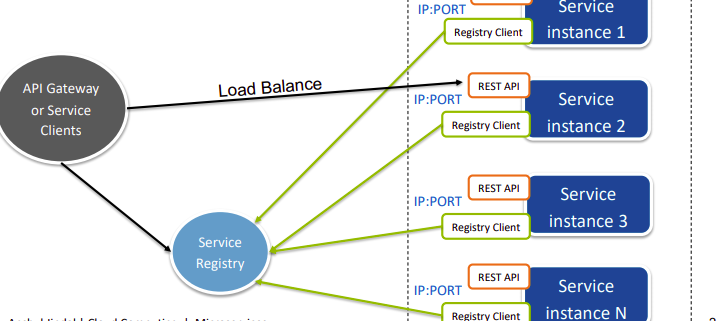
\includegraphics[width=0.7\textwidth]{client-side.png}
	\end{figure}
	
	
	\item \textbf{server-side} service discovery:
	\begin{itemize}
		\item an extra \textbf{load balancer}: it queries the registry and implements load balancing.
		
		$\rightarrow$ client has \textbf{no contact to service registry}
		
		$\rightarrow$ client \textbf{doesn't need to load balancing}
		
		\item Advantages:
		\begin{itemize}
			\item discovery abstracted away from client
			\item less code
		\end{itemize}
		Disadvantages: extra load balancer required
	\end{itemize}
	\begin{figure}[H]
		\centering
		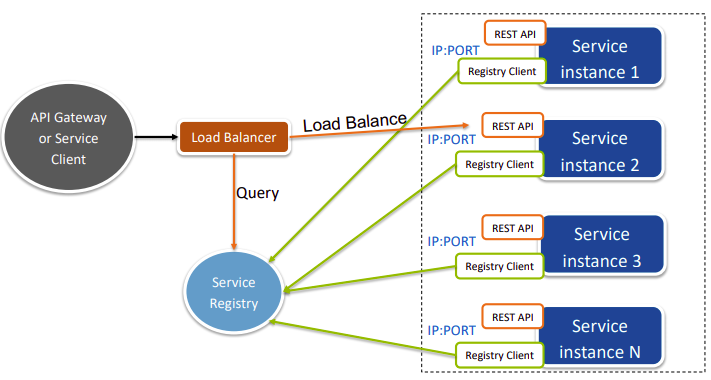
\includegraphics[width=0.7\textwidth]{server-side.png}
	\end{figure}
\end{itemize}

\subsubsection{Resilience -- Fault Tolerance Strategies}
\begin{itemize}
	\item basic request flow: 
	\begin{itemize}
		\item a user/load balancer sends a \textbf{request} to service and waits for a \textbf{response}.
		\item a \textbf{thread is assigned} along the request, in order to get data and send it back.
		\item when response is sent, the \textbf{thread is freed}. 
	\end{itemize}
	\begin{figure}[H]
		\centering
		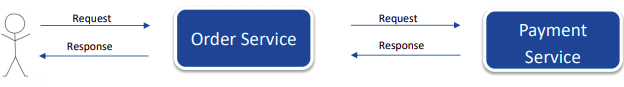
\includegraphics[width=0.8\textwidth]{request.png}
	\end{figure}
	\item \textbf{immediate failure}: fails at \textbf{request} (eg: connection refused) to service.
	\begin{itemize}
		\item possible reasons: overhead of requests
		\item solution: \textbf{try...catch}-code catches the error and returns error to client $\rightarrow$ thread is freed		
	\end{itemize}
	\begin{figure}[H]
		\centering
		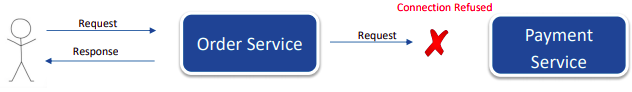
\includegraphics[width=0.8\textwidth]{immediate.png}
	\end{figure}
	
	
	\item \textbf{timeout failure}: fails at \textbf{response} from service to service. At high request rate, all threads are \textbf{waiting for response}, no free threads.
	\begin{itemize}
		\item possible reasons: service is overloaded or crashed
		
	\end{itemize}
	\begin{figure}[H]
		\centering
		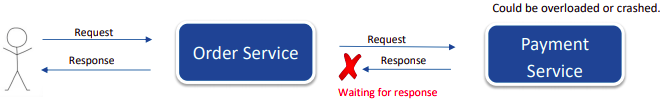
\includegraphics[width=0.8\textwidth]{timeout.png}
	\end{figure}
	
	\item \textbf{cascading failure}: due to timeout failure of one service instance to another service instance, this \textbf{timeout failure} is \textbf{propagated} to neighboured connected instances.
	\begin{figure}[H]
		\centering
		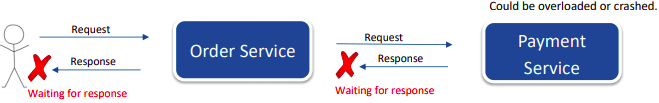
\includegraphics[width=0.8\textwidth]{cascading.png}
	\end{figure}
	\item Solutions to timeout/cascading failures: 
	\begin{itemize}
		\item timeout-value: returns error after timeout, thread is freed
		\item request interceptor/\textbf{circuit breaker}
		\begin{itemize}
			\item \textbf{intercepts all requests} from service to target service.
			\item \textbf{counter \& threshold implementation} of success \& failures. 
			\begin{itemize}
				\item closed: \#failures < threshold
				\item open: \#failures > threshold, default error response, thread is freed.
				\item half-open: remains open for a predefined sleep period and rechecks. 
			\end{itemize}
			\item checks regularly and refreshes.
		\end{itemize}
	\end{itemize}
	\begin{figure}[H]
		\centering
		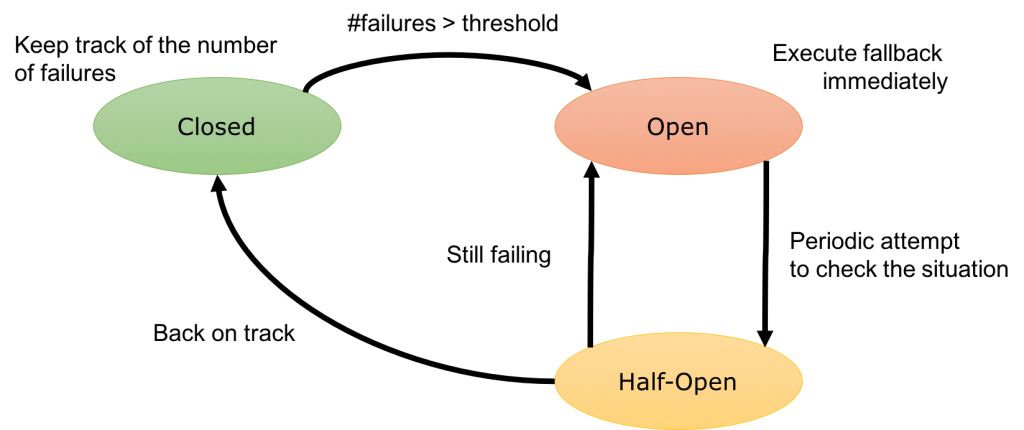
\includegraphics[width=0.7\textwidth]{circuit-breaker.png}
	\end{figure}
	
\end{itemize}

\subsubsection{Deployment Strategies}
\begin{itemize}
	\item \textbf{multiple service instances} per VM: service instances share resource of a VM together $\rightarrow$ for resource-efficient services
	\item \textbf{single service instance} per VM: for resource-hungry services
	\item \textbf{multiple service containers} per VM: each service instance is containerized with its needed libraries \& dependencies. $\rightarrow$ high portability, high scalability
	\item \textbf{single service container} per VM
\end{itemize}

\subsubsection{Rolling Updates Strategies}
\begin{itemize}
	\item Goal: implementation of updating of services.
	\item \textbf{Ramped-slow Rollout}: update in \textbf{rolling update} fashion. It \textbf{decreases old version} instances and \textbf{increases same number of new version} instances, until all old versions are removed.
	\begin{itemize}
		\item Advantages: 
		\begin{itemize}
			\item new version is slowly released across instances
			\item convenient for \textbf{stateful applications} that can handle rebalancing of data
		\end{itemize}
		Disadvantages:
		\begin{itemize}
			\item takes more time
			\item supporting mulitple APIs harder, if both versions use different patterns.
			\item no control over traffic, since load balancer directs request to either of the instances, it might follow wrong robin pattern.
		\end{itemize}
	\end{itemize}
	
	
	\item \textbf{Blue/Green}: new version of app is \textbf{deployed alongside} the old version. After testing new version, the load balancer will be \textbf{redirected} to send traffic to the new version. 
	
	\begin{itemize}
		\item Advantages:
		\begin{itemize}
			\item instant rollout/rollback
			\item no versioning issue (multiple versions coexist)
		\end{itemize}
		Disadvantages:
		\begin{itemize}
			\item requires double the resources. (same size of empty instances needed)
			\item requires testing before releasing, but still can't simulate the workload by client requests
		\end{itemize}
	\end{itemize}
	
	\item \textbf{Canary}: new version is \textbf{deployed and receives a subset of client requests} alongside the old version. We distribute the traffic amongst the versions by \textbf{adjusting the number of replicas} managed by a ReplicaSet.
	 After successful testing, all old versions are removed at one time.
	
	
	
	\begin{itemize}
		\item Advantages:
		\begin{itemize}
			\item version released for a subset of clients $\rightarrow$ testing of workload possible
			\item convenient for performance and error rate monitoring
			\item fast rollback 
		\end{itemize}
		Disadvantages:
		\begin{itemize}
			\item slow rollout: testing of workload, monitoring and improvement takes time
			\item fine tuned traffic distribution can be expensive. 
		\end{itemize}
	
	\end{itemize}
	
	\item \textbf{A/B Testing}: distribute traffic among versions \textbf{based on filter parameters} (weight, user, cookies). After successful testing, old versions are removed. 
	
	\begin{itemize}
		\item Advantages:
		\begin{itemize}
			\item intelligent load balancing
			\item full control over traffic distribution
		\end{itemize}
		Disadvantages:
		\begin{itemize}
			\item harder troubleshooting, distributed tracing of versions necessary
			\item additional tools needed
		\end{itemize}
		
		
		
	\end{itemize}
\end{itemize}

	\part{Monitoring and Autoscaling}

\section{Cloud Monitoring}

\subsection{Introduction \& Definitions}
\begin{itemize}
	\item Motivation: get data about the running system to make \textbf{best use of resources} at \textbf{lowest cost}.
	\begin{itemize}
		\item cloud infrastructure: resource management, root cause analysis, accounting \& metering, incident detection
		\item cloud applications: performance analysis, resource management, failure detection and debugging, SLA verification
	\end{itemize}
	\item Definition:
	\paragraph{Monitoring} the process of \textbf{collecting status information} of applications and resources to observe application and infrastructure.
	\paragraph{Monitoring System} components for gathering monitoring data at runtime -- \textbf{the target system(HW/SW), raw data and data storage}.
	\begin{itemize}
		\item requirements: comprehensive, low intrusion, extensibility, scalability, elasticity, accuracy, resilience
		
	\end{itemize}
	\paragraph{Target System} system to be monitored. an \textbf{online system}
	\begin{itemize}
		\item status depends not only on the \textbf{codes} but also the \textbf{environment} where it runs(\#VMs running on physical machines, bandwidth, cloud storage)
		
		$\rightarrow$ execution is \textbf{not reproducible}
		\item \textbf{real-time analysis} and \textbf{continuous data collection}
	\end{itemize}
	
	\paragraph{Analysis Tools} tools that read monitoring data from data storage.
	\paragraph{Informations}
	\begin{itemize}
		\item Alerts: alarm of exceeding thresholds. eg: CPU utilization 100\%, full storage
		\item Dashboard: overview of resources
		\item Costs: billing and usage of resources
		\item Bottleneck: most critical service/program that slows down response time/ most CPU time
		\item Root cause: once bottleneck defined, find out the root cause
		\item etc.
	\end{itemize}

	\paragraph{Blackbox Monitoring} \textbf{no data} are gained from \textbf{inside} of the monitored system(blackbox). A request interface, no visibility of internal system structure. eg: state of service like CPU/disk usage
	
	\paragraph{Whitebox Monitoring} data \textbf{also gained} from \textbf{inside} of the monitored system. eg: metrics specific to application \#requests
\end{itemize}

%\subsection{Metrics for Monitoring} \label{metrics}
%\begin{itemize}
%	\item Typical metrics:
%	\begin{itemize}
%		\item \textbf{latency}: response time
%		\item \textbf{throughput}: \#requests/sec, network I/O rate, concurrent sessions, \#transactions/sec 
%		\item \textbf{error rate}: rate of fail requests. 
%		\item utilization: CPU time/percentage, memory percentage, disk queue length(I/O)
%	\end{itemize}
%	
%	\item monitoring in different cloud layers:
%	\begin{figure}[H]
%		\centering
%		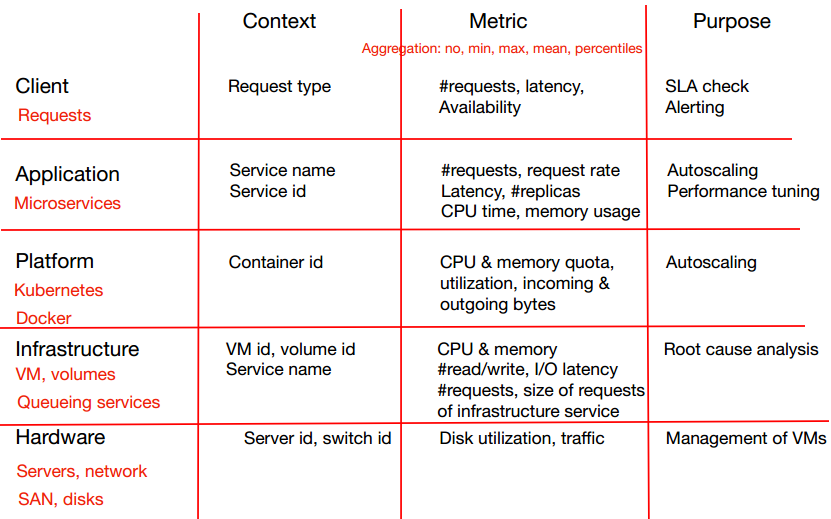
\includegraphics[width=\textwidth]{monitoring.png}
%	\end{figure}
%\end{itemize}



\subsection{Three Pillars/ Data Sources of Monitoring: Logs, Metrics, Traces}

\subsubsection{Logs}
\begin{itemize}
	\item Definition: a sequence of immutable records of discrete events.
	\item Characteristics:
	\begin{itemize}
		\item forms: plain texts, structured (eg: JSON), binary
		\item high level of detail, different levels possible
		\item hard to read and analyze
	\end{itemize}
	\item Techniques of Processing and Analyzing Logs: \textbf{ELK Stack}
	\begin{itemize}
		\item Beats \& Logstash: data ingestion. read, process logs and insert into Elastic Search.
		\item Elastic Search: search, analyze and store data
		\item Kibana: data visualization
	\end{itemize}
	\item Other providers: AWS CloudWatch Log Insights
	
\end{itemize}

\subsubsection{Metrics}
\begin{itemize}
	\item Typical metrics:
	\begin{itemize}
		\item \textbf{latency}: response time
		\item \textbf{throughput}: \#requests/sec, network I/O rate, concurrent sessions, \#transactions/sec 
		\item \textbf{error rate}: rate of fail requests. 
		\item utilization: CPU time/percentage, memory percentage, disk queue length(I/O)
	\end{itemize}
	
	\item monitoring in different cloud layers:
	\begin{figure}[H]
		\centering
		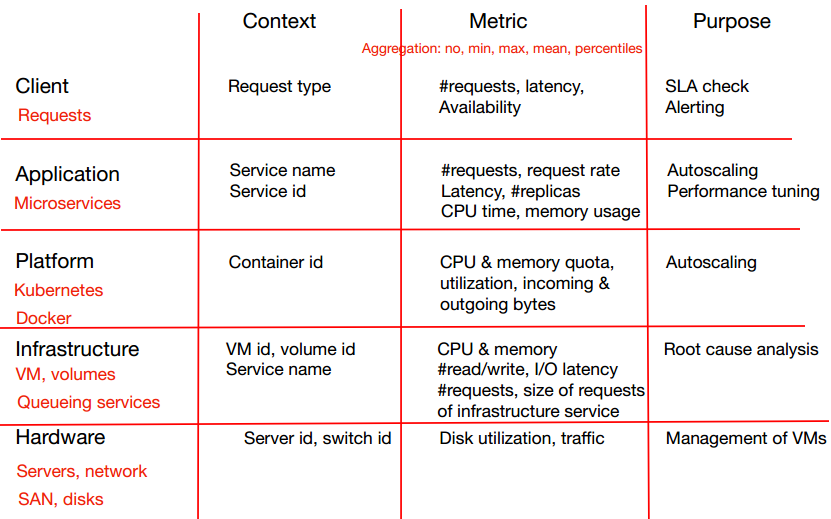
\includegraphics[width=\textwidth]{monitoring.png}
	\end{figure}
	\item Techniques for Processing and Analyzing Metrics: \textbf{Prometheus} (open source)
	\begin{itemize}
		\item data collection, storage \& querying: \textbf{time series} data
		\item Architecture:
		\begin{itemize}
			\item \textbf{server}: retrieved metrics saved in TSDB/storage, HTTP-server for data querying and analysis
			\item \textbf{target discovery}: define monitored targets 
			\item \textbf{metric retrival}: scraping at endpoint /metrics from target, pull for long-lived jobs, push gateway for short-lived jobs
			\item \textbf{alert manager}: receives alerts from server and send to various channels
			\item \textbf{data visualization}: Grafana
			
		\end{itemize}
		\item Scalability: \textbf{hierarchical}. Global DC stores aggregated data, local DC stores more detailed data.
		\begin{figure}[H]
			\centering
			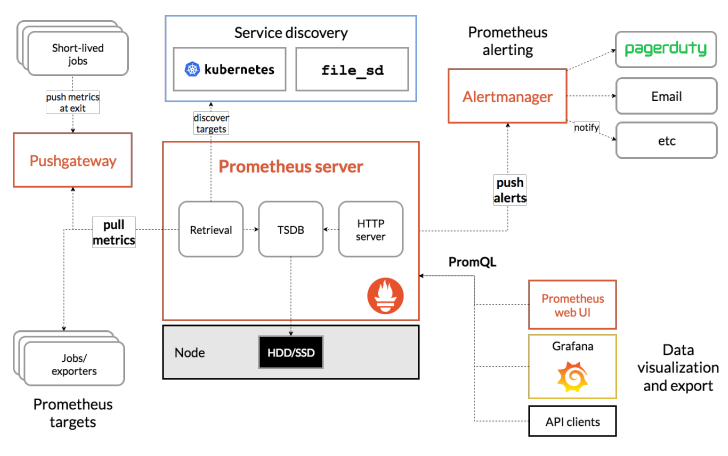
\includegraphics[width=0.8\textwidth]{prometheus.png}
		\end{figure}
		\item Other providers: AWS CloudWatch (custom and user-defined metrics)
	\end{itemize}
\end{itemize}

\subsubsection{Traces}
\begin{itemize}
	\item Definition: Finding out \textbf{interaction} of different services/events and \textbf{association of sequence}.
	\item Techniques for Processing and Analyzing Traces: \textbf{Google Dagger}
	\begin{itemize}
		\item \textbf{global request ID}: each event has a \textbf{trace ID} created at front-end service. It's \textbf{passed down} to subrequests.
		\item representation: \textbf{Dapper trace tree}
		\begin{itemize}
			\item nodes: \textbf{spans}, lifetime of a request. It has a \textbf{trace ID, parent ID and span ID}.
			\item edges: temporal relationship of calls
		\end{itemize}
		\item trace collection: logs --> dapper collectors --> into central bigtable(trace IDs and span IDs)
%	    \begin{itemize}
%	    	\item \textbf{span data} is written in local \textbf{log files}.
%	    	\item \textbf{dapper collector} reads files from all production hosts 
%	    	\item  \textbf{trace IDs and span IDs} are written to a cell in a \textbf{sparse Dapper Bigtable}
%	    \end{itemize}
	
	
		\item possible challenges: 
		\begin{itemize}
			\item clock skew from different servers in distributed system.
			\item \textbf{overheads}: caused by the massive amount of requests, trace generation and collection. Reduction by coalescing, adaptive sampling(application/trace id), asynchronous writes 
		\end{itemize}
		
		
	\end{itemize}
\end{itemize}




















\subsection{Challenges in Monitoring: Overheads}
\begin{itemize}
	\item Definition: overhead is any \textbf{combination of excess or indirect computation time, memory, bandwidth, or other resources} that are required to perform a specific task.  Such resource \textbf{doesn't contribute directly} to the result, but it's \textbf{required} to make it work.
	
	\item Reasons: 
	\begin{itemize}
		\item collection of data: \textbf{all available}
		\item instrumentation: insert additional binary calls/codes in the program and use these calls to trace native calls and achieve measurement goals
		\item aggregation computation
		\item memory overhead for buffering
		\item storage overhead for long-term storage
	\end{itemize}
	
	
	
	\item Reduction techniques: 
	\begin{itemize}
		\item reduce \textbf{number} of metrics: collect only important metrics
		\item reduce measurement \textbf{frequency}
		\item representation: choose \textbf{binary} instead of ASCII
		\item message \textbf{coalescing}: package multiple messages into one message
		\item \textbf{sampling}
		\item long-term \textbf{coarsening}: after some time period, only store \textbf{aggregated} values
	\end{itemize}
\end{itemize}





	\section{Autoscaling}

\begin{itemize}
	\item Motivation:
	\begin{itemize}
		\item \textbf{Scalability}: ability when resource $\uparrow$, application performance $\uparrow$, throughput $\uparrow$, latency $\downarrow$
		\item \textbf{Elasticity}: ability to \textbf{dynamically adapt}(up/down) the resource scale to the actual workload \textbf{without reboot}. 
		
		$\rightarrow$ No under-/overprovisioning, cost $\downarrow$, customer satisfaction $\uparrow$
		\item \textbf{Automation}: automatically, without interaction with the application owner
	\end{itemize}
	\item Capacity planning in cloud: avoid under-/overprovisioning by \textbf{dynmaic resource management} and \textbf{pay-per-use cost model}
\end{itemize}

\subsection{Scaling}

\begin{itemize}
	
	\item scaling performance: 
	\begin{itemize}
		\item speedup: $$\text{speedup(p processors)} = \frac{\text{performance(p processors)}}{\text{performance(1 processor)}}$$
		\item efficiency: $$\text{efficiency(p processors)} = \frac{\text{speedup(p processors)}}{p}$$
	\end{itemize}  
	\item scalabilty limit: restricted by \textbf{app design}, maximum \textbf{application capacity} or maximum \textbf{resource capacity}
	
	$\rightarrow$ scaling with infinite servers impossible
	\begin{itemize}
		\item \textbf{efficiency} of scaling \textbf{drops} when \textbf{more resources} are provisioned. $\rightarrow$ \textbf{bottleneck} of application gets dominant
		\item \textbf{poor application design} has lower scalability limit.
		\item more servers, communication latency increases.
	\end{itemize}
	\item resource to be scaled: \textbf{CPU (\#CPU, CPU time/percentage)}, memory, disk storage(size, bandwidth), network(throughput, bandwidth)
\end{itemize}

\subsubsection{Vertical Scaling -- Scaling Up}
\begin{itemize}
	\item increase capacity of a service instance by \textbf{increasing its allocated resources}. eg: CPU time percentage $\uparrow$, clock frequency $\uparrow$, cores $\uparrow$ 
	\item Advantages:
	\begin{itemize}
		\item no re-design of app required
		\item easy to replace, less management complexity
	\end{itemize}
	Disadvantages:
	\begin{itemize}
		\item powerful resources are expensive
		\item \textbf{limited} scalability due to resource capacity limit
	\end{itemize}
\end{itemize}


\subsubsection{Horizontal Scaling -- Scaling Out}
\begin{itemize}
	\item increase capacity of a service instance by \textbf{increasing the amount of same resources}.
	\item Advantages:	
	\begin{itemize}
		\item lower cost, implementation of commodity hardware
		\item larger scalability possibility (just increase the amount of resource)
	\end{itemize}
	Disadvantages:
	\begin{itemize}
		\item more management overhead
		\item distributed architecture required, load balancing, replica handling.
	\end{itemize}
\end{itemize}


\subsection{Autoscaling}

\begin{itemize}
	\item Goal: scale automatically to fulfill \textbf{Service Level Objectives}(SLO) while \textbf{minimizing costs}
	\begin{itemize}
		\item latency of request
		\item failed request rate
		\item service availability
	\end{itemize}
	\item Process: monitoring data --> analyzer --> scheduler takes scaling actions according to autoscaling policy --> executor gives cloud commands to scale up/down resources 
	\item Autoscaling approaches:
	\begin{itemize}
		\item \textbf{reactive}: \textbf{real-time} scaling according to policy(thresholds). detection of under/overloaded service
		\item \textbf{scheduled}: \textbf{periodical} scaling, time-stamped scaling events. eg: banking system, food ordering app
		\item \textbf{predictive}: predict future workload and scale \textbf{ahead of time}. It adapts proactively the \textbf{minimum} of autoscaling group.
	\end{itemize}
	\item Autoscaling implementation:
	\begin{itemize}
		\item \textbf{resource-centric}: scaling action directly modifies \textbf{resource allocation}(\#VM, CPU, memory, bandwidth). 
		\begin{itemize}
			\item Use-case: AWS Reactive Autoscaling -- scaling modifies \#VMs.
		\end{itemize}
		\item \textbf{service-centric}: scaling action directly modifies \textbf{\#service instances}. 
	\end{itemize}
	\item Autoscaling Policies (AWS):
	\begin{itemize}
		
		\item \textbf{target tracking scaling}: a \textbf{target value} of a \textbf{metric} is predefined, eg: CPU utilization at 40\%, \#requests per target at 1000. 
		
		Metrics that decrease when capacity increases and increase when capacity decreases can be used to \textbf{proportionally scale out or in} the number of instances using target tracking.
		\item \textbf{simple scaling}: scaling action is triggered based on metric, threshold or condition. 
		\begin{itemize}
			\item \textbf{cooldown period exists}: responses to \textbf{no additional alarms} until cooldown period expires, wait until scaling result visible and health check.  
		\end{itemize}
		\item \textbf{step scaling}: scaling action is triggered based on metric, threshold or condition with \textbf{step adjustments}.  The adjustments vary based on the \textbf{size of alarm breach}.
		\begin{itemize}
			\item \textbf{no cooldown period}: continues to \textbf{respond to additional alarms}, even while a scaling activity or health check replacement is in progress. Therefore, \textbf{all alarms that are breached are evaluated}
		\end{itemize}	
		
	\end{itemize}
\end{itemize}



\subsection{Load Balancing}
\begin{itemize}
	\item for \textbf{scaling out}(horizontal scaling)
	\item Goals:
	\begin{itemize}
		\item efficient resource utilization
		\item increase service availability (health check, restart nodes)
		\item increase aggregated capability of replicas $\rightarrow$ reduce response time and failure rate
	\end{itemize}
	\item Implementation: \textbf{multi-layer} load balancing
	\begin{itemize}
		\item different \textbf{layers} for different \textbf{functions}: service layer(request distribution), virtual machine layer(VM distribution), physical layer(server, CPU, storage, bandwidth distribution)
		\item \textbf{static VS. dynamic}: 
		\begin{itemize}
			\item static: scheduling according to \textbf{weighted round-robin}, \textbf{no feedback} about current load of servers
			\item dynamic: \textbf{feedback} from server to load balancer, able to adapt according to feedback.
		\end{itemize} 
		\item scalability: destributed design for load balancer
	\end{itemize}
	\item Algorithms:
	\begin{itemize}
		\item class-aware: \textbf{classification of requests} into sensitive, best-effort
		\item content-aware: direct \textbf{similar request content} to same server
		\item client-aware: based on \textbf{packet source}. Clients from similar area might share similar information, system can already \textbf{cache} the info.
	\end{itemize}
\end{itemize}


	
	
	% TODOS: REST API, container, orchestration, virtualization, docker VS. VM virtualization, hypervisor, service models, HPC & Cloud computing, VM migration, AWS availability, QoS, Kubernetes -- pods, minions, open source clouds, dockerfile, image file creation, Xeon Phi novel aspects, machine image, instance type, deployment models in microservice, lifecycle of VM, cost model serverless platform, infinite scaling, autoscaling approaches, step-scaling, normal read VS. strong consistent read, docker tag command
	
\end{document}
